%!TEX root = ../PhDThesis.tex



% *********************************************************************************************************************
\chapter{Studying talk around standalone VUIs in the home}\label{ch:empirical home}
% *********************************************************************************************************************



This final chapter of empirical data presents the study of conversations in households around the use of a voice-only \acf{VUI} device.
\iresubmission*[JR-3c, VV-2: Refocus the analysis on to the accomplishments of members in the setting]{The previous work in \autoref{ch:empirical cafe} explored conversations amongst groups of friends socialising together in a neighbourhood caf\'{e}, where conversations that included the use of \acp{VUI} on portable devices such as smartphones and tablets were the focus of the study, and of how this use was interleaved with the conversation.
The previous chapter demonstrated how accountable interactions with \acp{VUI} led to other users becoming involved in interactions with the device---this chapter further explores how interaction unfolds when that device is communal and all interaction with the device, including its response, is made accountable to those within the setting.
This chapter considers how interaction unfolds around a non-personal device (i.e. the device is `shared' amongst users in a multi-party environment), and without a screen (i.e. it draws entirely upon voice interaction to complete tasks).}

\iresubmission{To achieve the goal of this thesis, this chapter will study how families make use of a `smartspeaker' \ac{VUI} device in their home.
Given the variation in setting and interface being studied, this chapter adopts the approach taken with regards to data collection in the prior two chapters by recording audio from participant homes over a month-long period.}
%In order to consider how interaction unfolds when the interaction with the device is non-personal (i.e. the device is shared amongst users in a multi-party environment), and without a screen (i.e. it draws entirely upon voice), this chapter unpacks how interaction unfolds with the use of a `smartspeaker' device in homes.

This work was previously published and presented at the Computer-Human Interaction (CHI) conference\footnote{See \citet{Porcheron2018}.}\iresubmission[JR-3c: Refocus the analysis on to the key accomplishments of members in the setting]{---a number of changes have been made to address the research questions of this thesis}.
% ---a number of changes have been made This paper was awarded a `Best Paper' award at the conference, reserved for the top 1\% of papers submitted each year.



% *********************************************************************************************************************



\section{Introduction}\label{sec:empirical home introduction}
This chapter proceeds in the tradition of \acf{HCI} and \acf{CSCW} research that deploys technology to study the situated and emergent lived experience in the home~\citep{Tolmie2008a,Rooksby2015}.
In this way, the work continues upon recent work emerging in \ac{CSCW} that has begun to examine \acp{VUI} in collaborative action\footnote{As part of the PhD work, a workshop was organised at Computer-Supported Cooperative Work \& Social Computing conference on this topic, which went on to provide much insight and guidance for the work that was undertaken subsequently.
The workshop outline and focus is presented in the publication \citet{Porcheron2017a}.} for social settings such as meetings~\citep{McGregor2017}.
The study here reports findings from month-long deployments of the Amazon Echo with the `Alexa' voice agent in five households.
Audio capture was selectively performed by a separate device, a \acf{CVR}.
Over six hours of verbal exchanges involving the \ac{VUI} in some way were collected using this purpose-built device, 

\begin{revisedsubmission}
\label{line:prevhomestudy}A number of studies in homes, primarily focused on the use of mobile devices while another activity is taking place, have followed a variety of different practical approaches to data collection and focus.
For example, \citet{Schirra2014} used interviews to examine television watching and the use of Twitter, whereas \citet{Jokela2015b} employed a combination of interviews and diary studies.
More recently, \citet{Ferdous2016} incorporated home visits and self-controlled video capture of families' technology use during mealtimes.
In a similar vein to the approach taken by Ferdous, \citet{Rooksby2015} set up device screen capture technology on homeowners smartphones and installed video cameras in living rooms to capture television watching and the use of mobile devices---families were asked to turn these cameras on when they felt like it.
In this latter case, the analysis oriented to the sequentiality of action and methodically revealed how members routinely embed their use of mobile devices to enhance leisure time socialising around the television.
Both studies reveal crucial details about technology use in homes: that the home is a site for \textit{multi-activity} and that the use of technology fits into this as members engage in another activity while using a device and, in the case of television watching, as part of the same activity.
However, as will be discussed later in the chapter, practical and ethical issues preclude capturing video data or asking participants to assist in capturing data in this study.
Other approaches exist, such as relying on automatic devices logs from the \ac{VUI} device, as others have used (e.g. \citet{Ammari2019}), however this would have failed to provide access to the data this thesis needs: conversations around the \ac{VUI} itself.
Therefore, the study in this chapter adopts an approach used in other in-the-wild video ethnographic studies, such as by \citet{Pizza2016}, who created a secondary device to be used in addition to the device being examined, which captures and records the surrounding conversation to aid analysis but that does not require activating or controlling by the user.
\end{revisedsubmission}

Previously, how the use of voice-controlled interfaces, which have become a staple feature of commercially-available smartphones, tablets and other portable devices, are managed in conversation was explicated through the study of friends socialising in a caf\'{e}.
More recently, voice has become the primary interface with standalone screenless devices such as the Amazon Echo and Google Home.
These devices are marketed as `smartspeakers', are cylindrical in design (see \autoref{fig:empirical home introduction smartspeakers}), and are operated using voice only.
As with the \acp{VUI} found on portable devices, these devices are also referred to as `conversational agents', intelligent or virtual personal assistants, and so on.
Researchers have also adopted the term ``\textit{conversational} interfaces''~\citep[emphasis added]{McTear2016}, which resonates in many ways with the advertised user experience of such devices: specifically, these are technologies that it is possible to  `have a conversation' with, and which you can `just ask' questions.
In addition, the devices under study in this chapter are pitched as being especially suited for use in the home for a variety of purposes: to help with cooking, play music, access news and information, or play games.
Nevertheless, here the marketing- and perspective-agnostic term \acf{VUI} is used here in continuity with \autoref{ch:empirical cafe}.

\begin{figure}[bth]
    \subfloat[Amazon Echo]
    {\label{fig:empirical home introduction smartspeakers amazonecho}%
    
\includegraphics[height=6.6cm]{Graphics/3-3-Empirical-Home/Intro-AmazonEcho}} \quad \quad \qquad
    \subfloat[Google Home]
    {\label{fig:empirical home introduction smartspeakers googlehome}%
    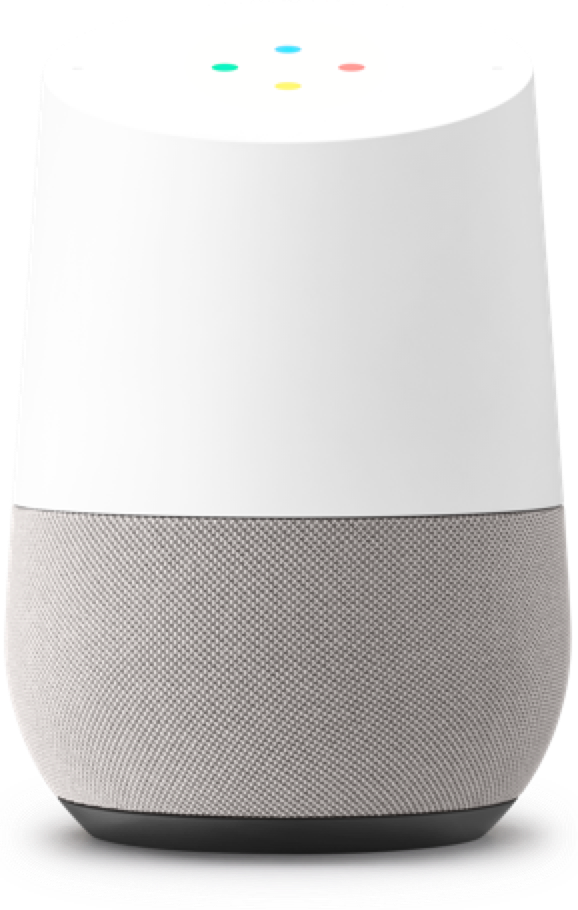
\includegraphics[height=4cm]{Graphics/3-3-Empirical-Home/Intro-GoogleHome}} \quad \quad \qquad
    \subfloat[Apple Homepod]
    {\label{fig:empirical home introduction smartspeakers homepod}%
    
\includegraphics[height=4.3cm]{Graphics/3-3-Empirical-Home/Intro-AppleHomepod}}
    \caption[`Smartspeaker' devices are typically self-contained cylindrical speakers designed for the home.]{`Smartspeaker' devices are typically self-contained cylindrical speakers designed for the home. The images of the Amazon Echo, Google Home, and Apple Homepod are copyright Amazon.com, Inc.; Google Inc.; and Apple Inc. respectively. Images of models available in 2017.}\label{fig:empirical home introduction smartspeakers}
\end{figure}

Despite the wealth of enabling research in computational linguistics such as natural language processing, dialogue systems, and computational sociolinguistics~\citep{Nguyen2016}, research that empirically examines the social and interactional issues of \ac{VUI} use in an everyday home setting is lacking.
In other words, with a few exceptions, little is known about the practical accomplishment of interactions that solely take place with \acp{VUI}, or the articulation of just how those interactions unfold in the everyday lives of their users.
The prior work in this thesis (see \autoref{ch:empirical cafe}) unpacked this interaction in relation to use that takes place when the device interaction involved a portable personal device with a touchscreen, however, here this chapter instead explores \iresubmission{how members of a home make use of a device} when the device use is done entirely using voice.
This absence of literature is significant since the work outlined here suggests a range of conceptual shifts that might need to be taken into account when designing \acp{VUI} for home settings and, more broadly, multi-party interactions.
This work goes on to reveal further details of collaborative efforts by members to get the device to work in and through everyday talk, in line with the research questions posed in this thesis.

%This study draws on the traditions of \acf{EMCA} (see \autoref{ch:background emca}) to examine various ways in which the \ac{VUI} was implicated in talk.

%In the main part of this study, the ways in which the \ac{VUI} is embedded into the situational exigencies of the home are explored (such as other activities going on during use), and how its users account for the interactional work that this use involves.
%This chapter then moves on to look at the sequentially organised ways in which \ac{VUI} use is achieved in a multi-party conversational setting, and then concludes by discussing three key issues emerging from the findings: conceptual concerns regarding the framing of \ac{VUI} as `conversational' interaction; the ways that requests to \ac{VUI} are designed and the implication of accountability for this; and finally, the design of \ac{VUI} responses, and considering their role as interactional resources that users `go on' with.



% *********************************************************************************************************************


% \section{Research questions}\label{sec:empirical home rqs}
% This work, thus far, has unpacked numerous cooperative and collaborative activities around the use of portable touchscreen-based devices in casual-social settings.
% Such examples have included how members accountably sustain device use in and through conversation (\ref{sec:empirical pub discussion coop}) and the mutual production of silence following a request to a \ac{VUI} (\ref{sec:empirical cafe findings collab}).
% Here, this work moves onto considering how interaction unfolds in situations where voice is the only mode of interaction with the device.
% Furthermore, this work differs insomuch that it explores the use of devices as part of ongoing activities, i.e. this study will unpack how the use of \acs{VUI} is achieved and embedded within home life as multiple members of the have gathered:

% \PrintRQ{1}
% \PrintRQ{2}

% Furthermore, drawing upon RQ2, this work will go on to reveal further details that are explicated from the data of how members collaborate with each other.
% These \ac{VUI} devices under study embody two key characteristics that will impact how interaction with and around the device unfolds: (1) the devices pivot from being singularly controlled and owned by a single member to a communally controlled device controlled through any voice, where all members in the household can freely use the device, and it is owned by the household; and (2) the device does not provide a screen to denote how a prior request `went wrong', something that was used by members in their interaction with the device to resolve trouble (see \autoref{sec:empirical cafe findings multimodality}).



% *********************************************************************************************************************



\section{Study design}\label{sec:empirical home design}
\begin{revisedsubmission}[JR-2b: Include detail on the choice of setting and its connection to the technology use under study]
A brief description of the setting in which the studies were undertaken is provided below, including details about the participants involved.
This study deviates from the modus operandi established in the prior two empirical chapters in that the collection of data in this study is an audio-only longitudinal study in a non-public setting.
This section will introduce the rationale for this design as well as the reasoning for the continued adoption of an ethnomethodological analytic orientation (see \autoref{ch:background approach}).
The study was approved by the university's School of Computer Science Research Ethics Committee.
\end{revisedsubmission}



% *********************************************************************************************************************



\subsection{The home a study setting}\label{sec:empirical home design setting}
\begin{revisedsubmission}[JR-2b: Include detail on the choice of setting and its connection to the technology use under study]
Whereas the studies in Chapters \ref{ch:empirical pub} and \ref{ch:empirical cafe} focus on studying interaction in a semi-public `casual-social' setting (a pub and a caf\'{e} respectively), this exploration of standalone \acp{VUI} is conducted in participants' homes.
This is driven by the design of the device under study---whereas smartphones are engineered to be portable devices that allow users to achieve tasks irrespective of their location, `smartspeakers' are typically not designed to portable, need to be plugged in to mains electricity\footnote{Some portable standalone smartspeakers have since been released, such as the Amazon Tap, although none were available at the time of study and the Amazon Tap has since been seemingly discontinued.}, require configuration using an app to connect to a Wi-Fi connection, and are typically pitched by manufacturers as devices for the home.
With smartphones, their portability affords their use and thus the possibility of \textit{studying interactions around their use} in a range of different venues, with the ones chosen done so to explore how devices are used and interleaved within a multi-party conversation of friends socialising in a relaxed manner in a setting perspicuous to their use.
However, \acp{VUI} are not marketed as portable or \textit{personal}, but instead as communal devices that can be `installed' in a fixed location in the home, and usable by any person living in---or passing through---the space.

Despite the differences in design, including the lack of \acf{GUI}, the concept of the \ac{VUI} on a standalone device intersects with that of the \ac{VUI} on the smartphone: users use a `hotword', they deliver their request `using natural language'\footnote{This phrase is in quotes because its veracity is not established but proclaimed in the marketing materials of device manufacturers.}, and the \ac{VUI} responds through a synthesised voice that sounds humanlike\footnote{Relatively speaking, to an untrained ear, and within limits.} (note that in the case of smartspeakers, this synthesised voice is always produced whereas it is optional on portable devices).
Therefore, the lack of portability, personalness to an individual, and no \ac{GUI} establish the smartspeaker as a distinct but interrelated product to \acp{VUI} on smartphones, and establishes the need for studying the use of such a device in a home environment.
\end{revisedsubmission}



% *********************************************************************************************************************



\subsection{Collecting data in the home}\label{sec:empirical home design data}
In order to capture naturalistic use of a \ac{VUI} in the home, five households were recruited to take part in a month-long longitudinal study. 
\iresubmission*[J2-2b: Include details on the pertinence of the setting and technology choice]{The desire to adopt month-long longitudinal study approach instead of observing a gathering of friends as in the prior two studies stems from the both the design of \ac{VUI} smartspeakers being pitched as home-based devices and the recentness of the introduction to market of standalone smartspeakers.
While smartphones had been around for more than six years at the time of study in \autoref{ch:empirical pub} and \acp{VUI} had been found on smartphones for more than three years at the time of study in \autoref{ch:empirical cafe}, smartspeakers were less than two years old, and in the UK less than one year old at the time of this study.
A longitudinal study would potentially allow users to configure and develop \textit{some} competency in using the \ac{VUI} device rather than only focusing on their first encounters with a device\footnote{The only real requirement was that users had developed enough competency to be able to use the device, no measure of competency was taken or sought as the goal was not to determine or evaluate use over time.}.
}

Of the five households recruited for the study, three were inhabited by couples, while two households were families consisting of two parents and two children.
The age range of the adult participants spanned from late-20s to mid-50s.
Each participating household was given an Amazon Echo, configured with a household member's personal Amazon account, and the Alexa companion app was installed on one of their personal smartphones.
\iresubmission*[J2-2b: Include details on the pertinence of the setting and technology choice]{The purpose of this is to identify how the conversations unfold around the use of the \ac{VUI} in the designers' intended setting.}
Households freely selected the positioning of their Echo and could relocate it when and as desired.
Four of the households placed the \ac{VUI} in a kitchen or dining area, while one placed it in a living room.
\icorrection*[Added  reference to activity centres]{\label{line:activitycentres}These sorts of places, through the presence of the \ac{VUI} smartspeaker, are made into \textit{activity centres} and thus \textit{ecological habitats}.
\citet{Crabtree2003} define the former as ``places where media are actively produced and consumed and where information is transformed''~\citep[p. 215]{Crabtree2003} and the latter as ``places where communication media live and where residents go in order to locate particular resources''~\citep[p. 215]{Crabtree2003}.
The multiplicity of functions proffered by \acp{VUI} facilitates household members to make these devices `at home' (i.e. for their use to be part of the routine lived experience of those in the home rather than of some unusual occurrence)---to produce and consume media, as well as a site for communication\footnote{Although the Amazon Echo does include features for communication, such as voice calling, none was observed in these studies, perhaps given the relative nascency of the devices in the UK.}.}
%This chapter will reveal how the Echo is made at home as an \textit{activity centre}.}


\subsubsection{The Conditional Voice Recorder}\label{sec:empirical cafe design data cvr}
\begin{revisedsubmission}[J2-2b: Include details on the pertinence of the setting and technology choice]
Given the sensitivity and technical/ethical challenges of collecting data in the home over an extended period, this study further deviates from the previous studies by opting for audio collection only instead of video.
It was considered that recruiting participants to allow video capture in their home for an extended period would generate vast amounts of video data, including of many moments participants did not want to be recorded, as well as potentially being an invasive way of collecting data.
Solutions to this were considered, such as requiring participants to start and end recording, however, this would potentially impede the capture of any spontaneous interactions with the \ac{VUI} device.
Therefore, given the desire to study interaction in the home over a month-long period, this study further specifies that only interactions temporally close to the use of the \ac{VUI} should be studied, given the sensitivity to---and infeasibility of---analysing all interaction in the home.
\end{revisedsubmission}

To capture the use of the Alexa \ac{VUI} in the home, a second purpose-built device---termed the \acf{CVR}---was \iresubmission{designed, built, and} deployed with the Amazon Echo.
The \ac{CVR} is activated when a proximate Echo is used (the design of the \ac{CVR} is depicted in \autoref{fig:empirical home desig cvr}) by continually capturing audio using a conference microphone, i.e. it records voice \textit{conditionally} upon some event occurring.
The device always keeps the last minute of audio in a temporary buffer in the non-permanent memory of the device while active.
When the hotword, `Alexa' (that activates and begins the use of the \ac{VUI}) is detected, the \ac{CVR} saves the prior minute into permanent storage and records one further minute of audio (this period is extended if the hotword is heard in the subsequent minute).
The \ac{CVR} also features a button to turn off audio capture, and two LEDs (blue and red), that indicate when the \ac{CVR} is `listening' for the hotword (blue) and when it is recording (red).
The \ac{CVR} is more sensitive than the \ac{VUI}\footnote{Voice recognition systems often have an accuracy or threshold variable that allows a `best guess' of whether a particular sound fits a given word or not. In this case, the \ac{CVR} was prone to false positives such that it may sometimes activate recording when the user had not uttered the hotword. This was seen as favourable to false negatives, where the \ac{CVR} would not activate when the \ac{VUI} was used.}, to ensure talk to Alexa was captured.

\begin{figure}
    \centering
    \includegraphics[width=.7\textwidth]{Graphics/3-3-Empirical-Home/Design-ConditionalVoiceRecorder}
    \caption[External design of the Conditional Voice Recorder (CVR).]{The Conditional Voice Recorder (CVR) is a small (12cm by 12cm) black box with a white lid. On the lid is a conference microphone, two LEDs (one blue, one red; to indicate when the \ac{CVR} is actively 'listening' for the hotword and when it is recording, respectively), and a button to turn on, or off, the CVR. Pictured also is the bottom part of an Amazon Echo. Version 2 of the \ac{CVR} is shown (Version 1 being an initial developmental prototype).}\label{fig:empirical home desig cvr}
\end{figure}



% *********************************************************************************************************************



\subsection{Analysing the collected data}\label{sec:empirical home design analysis}
\iresubmission[JR3a, ER-G1: Add further information about the analysis of the corpus, including the selection of fragments]{The resulting corpus of data from the deployments consists of over 6 hours of recorded data, where each audio clip consists of one or more requests to the \ac{VUI} in the home, as well as the preceding and succeeding conversation around the request.}
Overall, 883 distinct `request' utterances have been identified, where a request is talk that is directed to the \ac{VUI} in a seeming attempt to get it to `do something', e.g. answer a trivia question, play particular music, or set a timer.
Often these requests formed part of a larger sequence which might encompass various other requests that are temporally and/or topically related.
The corpus contains 185 of these (i.e. there are 185 audio clips containing the use of the \ac{VUI}).

\begin{revisedsubmission}[JR-3a: Change EMCA to `study informed by EM']
As with the previous chapters, this work takes on the perspective of ethnomethodology and is interested in how members organised their actions with and around the \ac{VUI}.
Specifically, this work examines how members, as conversationalists, analysed moment-by-moment unfolding interactions with and around the device and with one another to accomplish and address the problem that occasioned the use of the \ac{VUI}.
\end{revisedsubmission}

\iresubmission*[ER-G1: Add further information about the analysis of the corpus, primarily the selection of fragments]{A substantive review of the audio clips was performed to document the requests to the \ac{VUI} and who made them.
Twelve fragments were then transcribed carefully using the Jeffersonian transcription system (see \appref{app:notation}).
These fragments were selected in line with the aims of this research to reveal the ways in which members use a standalone \ac{VUI} device in and through conversation (in other words: each clip focused on the use of the \ac{VUI} while other people where audibly co-present).
Although there was interest in situations where the \ac{VUI} was used solitarily, this is beyond the focus of this thesis' aim to study the use of technology during gatherings of multiple people and of the naturally accountable interactions around this use (see~\ref{line:naturalaccountability} on natural accountability).
It was determined that each fragment selected warranted further investigation, with each fragment being reviewed individually and discussed collaboratively with other researchers multiple times.
The fragments selected for inclusion in this thesis `vividly exhibit'~\citep{Bannon1993} the interactional accomplishments of the members in selecting to use the \ac{VUI}, as exemplars of the data in the corpus~\citep{Crabtree2012}, but are not representative of how all instances of \ac{VUI} use may unfold.}

%Based on the findings in \autoref{ch:empirical cafe}, it was expected that various conversational methods would come into play and be adapted so as to `get stuff done' with the \ac{VUI}.
%The use of \acf{VUI} as a tool for unpacking the sequential and embedded practice of situated actions is an established technique in \ac{HCI} (e.g. \citet{Gilbert1990}), but it is noted that this work does not seek to treat the device as a \textit{participant} in conversation (see the discussion in the prior empirical chapter, \ref{sec:empirical cafe discussion humanlike}).

%The fragments of data presented in this chapter draw upon the transcript notation in \appref{app:notation}.
All names and identifiable information within the transcripts are, as before, entirely fictional.
%Some counting is provided throughout the findings to give an understanding of the commonality for which different aspects of \ac{VUI} use occurred.
%However, these should be treated as descriptive indices and not quantitative findings.
Talk that appears primarily to be addressed to the \ac{VUI} by members of the setting is highlighted in bold text.
In turn, the synthesised voice produced by the \ac{VUI} is identified by the label `ALE' (i.e. ALExa) in transcripts.
The inclusion of synthesised voice output as part of the transcript should not be seen to suggest any conceptual equivalence among members and the \ac{VUI}, but merely constitutes a convenient way of presenting the temporal organisation of device output as it appears in interaction.

%The fragments examined in this chapter are taken from one family living together in a household, and in particular, during their use of the \ac{VUI} while consuming family meals.


%Inspired by a similar line of approach to \citet{Reeves2016}, this work looks at the family's interactions in two interconnected ways.
%Firstly, the ways in which the \ac{VUI} is made `at home' and embedded into the various activities of home life are examined.
%Secondly, this chapter turns to unpacking how the \ac{VUI} features in \textit{sequential courses of action}, i.e. the orderly production of conversation.



% *********************************************************************************************************************



\section{Findings}\label{sec:empirical home findings}
\iresubmission[JR-3a, JR-3c: Introduce the fragments, two of which are different to the prior submission]{Data from the fieldwork will now be introduced and presented over a series of data excerpts. %---these fragments are \textit{vivid exhibits}~\citep{Crabtree2012} of the data within the collected corpus.
The fragments revealed in this chapter are taken from two different households over three different occasions.
The first fragment examines how users test the \textit{functionality} of a \ac{VUI}, as per \ref{sec:empirical cafe findings capability} with smartphone-based \acp{VUI} (see \ref{sec:empirical home findings capability}), and provides a clear sense of the nature of interaction with a \ac{VUI} device.
The second further introduces how the use of a screenless-\ac{VUI} device is done accountably to the normative moral order of the setting, in this case to ask for background music suitable to a New Year's Eve party.
Whereas the first fragment reveals little of the social interaction around the \ac{VUI}, this second fragment  progressively emphasises the intricate nature in which \acp{VUI} are used, with the different sorts of activities that take place around their use.
The third fragment introduced in this chapter reveals how the design of a \ac{VUI} smartspeaker supports their use for long-running activities while those collocated are also performing another task together (in this case, eating a family meal while playing a game together), bringing in the richness of the setting and how \ac{VUI} devices are used as part of the multi-activity home.}
Interaction with the device will be shown not to take place as a singular indiscriminate event but rather is achieved as a situated action as part of---or rather, \textit{interleaved} within---the already ongoing activities that unfold within the home.
\begin{revisedsubmission}[ER-G1: Add further information about the analysis of the corpus, primarily the selection of fragments]{
In this sense, and by design, the home is regarded as---and will be shown to be---a perspicuous setting~\citep[p. 181]{Garfinkel2002} for the use of \ac{VUI} devices and thus the examination of their use.}

%\appref{app:notation} provides details of the transcript notation used in this thesis.
%All names and identifiable information within the transcripts provided are entirely fictional.

%The family are selected for analysis as a single case~\citep{Schegloff1987} to provide a series of ``vivid exhibits''~\citep{Bannon1993} of the broad array of methods members employ across the corpus.

As before in the prior empirical chapters, this work is not interested in claiming that these are `representative' or `generalised' findings of how all interactions can or may unfold; rather, it is given that members continually try to make their own interactions orderly and rely upon the orderly features of others so as to each analyse what the others are doing and thus `go on' (the \textit{ethnomethodological perspective}, see~\autoref{ch:background approach}).
This means that this chapter, as with the prior two, seeks to exhibit how members bring the \ac{VUI} device practically into that interaction order.
\end{revisedsubmission}



% *********************************************************************************************************************



\subsection{Establishing the capability of a VUI}\label{sec:empirical home findings capability}
\begin{revisedsubmission}[JR-3a, JR-3c: This section is new, constructed from previously collected data]
This first fragment, called \textit{Where is Greece?}\footnote{The complete fragment is included in \appref{app:fragments-home greece}.}, commences in \autoref{frag:empirical home findings capability-i}.
This excerpt unfolds as the two homeowners, Nikos and Isabel, are entertaining their neighbours, Leah and John, who are chatting and socialising around the bar in the kitchen area of their flat.
Nikos introduces the Amazon Echo and then Leah and John take turns using the device, asking it various questions.
%We join the action as Leah asks ``where is greece?'', establishing her request to determine how a device without a screen responds to requests for the location of places.
All participants in the conversation are Greek, and at times converse in Greek and sometimes in English (primarily towards the Amazon Echo).
Talk that was Greek in these conversations was translated into English by Nikos following the study.

Previously, in \ref{sec:empirical cafe findings capability}, establishing the functionality of a smartphone-based \ac{VUI} was shown to consist of two actions by members, and indeed the same actions are revealed to take place with the screenless \ac{VUI} device when unpacking the actions of members:
\begin{enumerate}[label=(\roman*)]
\item \nameref{sec:empirical home findings capability establish}, and
\item \nameref{sec:empirical home findings capability testing}.
\end{enumerate}

These activities are now explicated in the following two sections, revealing the problem case of whether the device is able to deal with requests for the details of places.
\end{revisedsubmission}



% *********************************************************************************************************************



\subsubsection{Establishing the desired function}\label{sec:empirical home findings capability establish}
\begin{revisedsubmission}
We join the action in \autoref{frag:empirical home findings capability-i} as the friends are sitting down to drink coffee in the kitchen area of the flat.
John, one of the guests, has asked a number of questions to the device regarding definitions of words, a well-advertised feature of the Amazon Echo.
After requesting a few words, Leah takes a turn in conversation and introduces a request for a different type of request: one for details of a specific location.
\end{revisedsubmission}

\begin{inlinefrag}
    {\fragresubmission{JR-3c, ER-H: This is a new fragment from the existing corpus}
    \begin{transcript}
        \by LEA {\textbf{alexa (.) where is greece}} \\
        \later   {2.0} \\
        \by ALE {\textit{// greece is a un-recognised country in the northern hemisphere}} \\
        \by     {\textit{(.) it shares a border with turkey, albania, bulgaria}} \\
        \by     {\textit{and macedonia= //}} \\
        \by ISA {~~~~~~~~~~~~~=[ that’s it ]} \\
        \by LEA {~~~~~~~~~~~~~=[ that’s it ]} \\
    \end{transcript}
    \caption{Where is Greece? (i)}\label{frag:empirical home findings capability-i}
    }
\end{inlinefrag}

\begin{revisedsubmission}
In this opening excerpt, Leah makes the request to the \ac{VUI} for \QF[01]{where is greece?}.
Given the \ac{VUI} is screenless, this request is positioned not as a `show me on a map', but rather a request for a description of the location of the country Greece.
The members do not talk as the \ac{VUI} delivers its response, listing the neighbouring countries of Greece and upon the device remarking that Greece neighbours Macedonia, both Isabel and Leah simultaneously remark \QF*[06--07]{that's it}.
All four friends in the room, of course, \textit{know} the location of Greece---as they are all Greek---the request is merely to explore the capability of the device to support sense-making in how the device responds to various requests.
The remark of \QF{that's it}, delivered jointly by Leah and Isabel latches on the completion of the name \QF[05]{macedonia} by \ac{VUI}, and turns upon a geopolitical dispute between the nations of Greece and the Republic of Macedonia, and brings to the fore how members of the setting are waiting for the name to be produced as part of the list of neighbouring countries\footnote{This was verified through discussion with the participant household members following the study.}.

In performing this request, Leah establishes the premise that her request is to test the capability of the \ac{VUI} to respond to questions about the location of places.
In choosing to request details of a location of which she is acutely aware, she reveals that her request is both to determine whether the device supports \textit{this kind of request}, and further enable her to establish the veracity of the response from the \ac{VUI}.

Of course, Leah does more than establishing the desired function of the \ac{VUI}, she \textit{tests} its functionality too, by addressing the device with her request.
In other words, Leah's address to the \ac{VUI} performs both the work of \textit{establishing} and \textit{testing} it.
The next section expands upon the notion of testing a \ac{VUI} by examining two further questions put to the device.
\end{revisedsubmission}



% *********************************************************************************************************************



\subsubsection{Testing the functionality by addressing the VUI}\label{sec:empirical home findings capability testing}
\begin{revisedsubmission}
Following Leah's opening request to establish and question the device to give information regarding the location of places, John proceeds to ask a further question in the same vein.
In this next exhibit, found in \autoref{frag:empirical home findings capability-ii}, John asks the \ac{VUI} for the location of \textit{Amfissa}, a city in Greece.
\end{revisedsubmission}

\begin{inlinefrag}
    {\fragresubmission{JR-3c, ER-H: This is a new fragment from the existing corpus}
    \begin{transcript}[9]
        \by JOH {\textbf{alexa where is amfissa}} \\
        \later  {2.0} \\
        \by ALE {\textit{// amfissa is a city in phocidos (..) greece (.) it is 82 miles}} \\
        \by     {\textit{133 kilometres west of athens and 26 miles 42 kilometres south}} \\
        \by     {\textit{of lamia //}} \\
    \end{transcript}
    \caption{Where is Greece? (ii)}\label{frag:empirical home findings capability-ii}
    }
\end{inlinefrag}

\begin{revisedsubmission}
In this second excerpt, John follows the same structure in his request to the device as Leah (i.e. \textit{where is\ldots}), but this time asks for the location of a city in Greece, and could be considered to be `upping the ante' by asking a question that is ostensibly more difficult given its specificity of being a city rather than country.
In this instance, as with the prior request, the device responds seemingly correctly with the members in the setting allowing the device to complete its response.

Following this response, John makes a further attempt at \textit{testing the functionality of the \ac{VUI}}, as depicted in \autoref{frag:empirical home findings capability-iii}.
As before, he does this by following the same format of request as established by Leah (i.e. \textit{where is}), but this time opts to ask the \ac{VUI} device for the location of \QF[15]{delphi}\footnote{This is spelt \textit{delph-ee} in the fragment transcript to distinguish it from the different pronunciation used by the \ac{VUI} device in its response of \textit{delph-i}.}.
\end{revisedsubmission}

\begin{inlinefrag}
    {\fragresubmission{JR-3c, ER-H: This is a new fragment from the existing corpus}
    \begin{transcript}[15]
        \by JOH {\textbf{alexa where is (0.3) delph-ee}} \\
        \later  {7.0} \\
        \by ALE {\textit{// delph-i is a village in carroll county indiana (.) indiana (.)}} \\
        \by     {\textit{it is 62 miles 99 kilometres north of Indianapolis and 87 miles}} \\
        \by     {\textit{140 kilometres= //}} \\
        \by NIK {~~~~~~~~~~~~~~~\textbf{=alexa stop}} \\
    \end{transcript}
    \caption{Where is Greece? (iii)}\label{frag:empirical home findings capability-iii}
    }
\end{inlinefrag}

\begin{revisedsubmission}
In the first excerpt in this fragment, Leah asks the \ac{VUI} device for the location of \textit{Greece}, the country she and other co-interlocutors are from.
In this, she establishes her desire to determine how the device provides information about the location of places and chooses a place of which she is aware---in this case, her country of origin.
This notion is further realised through the successive utterances produced in the setting (the retrospective-prospective character of action, see \ref{sec:background approach em sequentiality})
The second request to the \ac{VUI} smartspeaker, by John, her partner, further tests the \ac{VUI} by increasing the specificity of the locale put to the device to locate.
In both cases, ostensibly, the device responds as members seemingly expect.
In this final excerpt, John asks for the location of \QF[15]{delphi}, which is an ancient monument and a registered UNESCO World Heritage Site in Greece.
With this, it seemingly becomes evident that John's follow up question is asking for the location of something more precise than the prior two questions (country and then city), and further establishes the ratcheting of specificity over the three requests to the device in this fragment.

After John's request, the \ac{VUI} device takes 7 seconds to respond, during which the members remain quiet\footnote{Given \acp{VUI} devices of this nature do not verbalise what-it-is-doing, it is unclear as to the cause of this elongated time between request and response.}.
The device begins responding, and commences its response with a different pronunciation of the place requested by John (delph\textit{ee} vs. delph\textit{i}), and gives the location of a village in Indiana, USA.
Given the coherence and context established through the production of the prior two requests to the device, it is determined that this response from the device is not the intended location of which John was seeking details.
Nikos cuts the \ac{VUI} device off as it continues to produce information about Delphi, Indiana by producing the request \QF[20]{alexa stop}.%---the group stop using the device to get the details of locales.

The group discussion then moves on to new topics after this response, affirming this sequence of events was around the purpose of \textit{testing the functionality of the \ac{VUI}} rather than actually seeking information about the location of a country, city, and landmark.
With smartphone-based \acp{VUI}, establishing the capability of the \ac{VUI} was positioned as a case that deviated from actions performed typically with touchscreen-based devices, as the \ac{VUI} features were made available to users in the past few years.
Moreover, in the context of the screenless devices, which were released within the UK within the prior three months before the recording of this fragment occurred, establishing the capability of the \ac{VUI} was a recurrent practice amongst all the households studied.
\end{revisedsubmission}



% *********************************************************************************************************************



\crpagebreak\subsubsection{Methodical accomplishments in this fragment}\label{sec:empirical home findings capability methods}
\begin{revisedsubmission}
In this first fragment, the work of establishing the capability of a smartspeaker \ac{VUI} to respond to \QF{where is} questions is unpacked.
Leah initially opens the \textbf{address to the \ac{VUI} by using the hotword, followed by her request}.
Through the member's perspective, this request is establishing and testing the functionality of the \ac{VUI}, given that Leah knows the answer to the question.
The \ac{VUI} computes a response for a few seconds, and the co-present members \textbf{do not talk until the \ac{VUI} has fully delivered its answer} through a synthesised voice.
A second request is produced by another member through \textbf{address to the \ac{VUI}}, using the same wording but with a more specific location (i.e. a `harder' question, and again this turns upon the members of the setting being knowledgeable of the correct answer).
Again, the \ac{VUI} computes and responds to this request through the synthesised voice.
A third request that is ostensibly more difficult again is \textbf{addressed to the \ac{VUI}} by the same member.
The \ac{VUI} takes seven seconds to compute an answer and begins to deliver its response, using a different pronunciation of the locale given by the user.
The coherence of the questions establishes that this answer from the \ac{VUI} is `incorrect' (i.e. for a different location with the same spelling), and is reinforced by another member of the setting \textbf{cutting off the \ac{VUI}'s response delivery by addressing it with a stop command}.
Through the perspective of the members, this sequence of requests is about establishing and testing the capability of the \ac{VUI}---not to literally find the location of Greece, Amfissa, and Delphi.
The interactional project was a success from this perspective.
\end{revisedsubmission}



% *********************************************************************************************************************



\subsection{Asking the VUI to play music}\label{sec:empirical home findings music}
\begin{revisedsubmission}[JR-3a, JR-3c: This section is new, constructed from previously collected data]
This second fragment, called \textit{New Year's Music?}\footnote{The complete fragment is included in \appref{app:fragments-home nye-music}.}, commences in \autoref{frag:empirical home findings music-i}.
This excerpt unfolds as the same two homeowners as above, Nikos and Isabel, are hosting a New Year's Eve party.
The party has been going for some time and during a conversation about the Amazon Echo and the \ac{CVR}, an attendee commences the interactional project of playing some background music using the Amazon Echo.
One of the key marketed features of the Echo is the ability to perform long-running tasks such as playing music or setting timers.

In this fragment, a guest, Anna, will be facilitated in making a request to the device by Nikos, however, the request ultimately fails and the two users attend to dealing with the outcome of the device's computation.
This fragment will progressively demonstrate the ways in which interaction with a \ac{VUI} occurs within and is accountable to others within the setting.

Overall, the members' problem of getting the device to play music in the background will be shown to consist of two core activities that will be unpacked across a number of excerpts:
\end{revisedsubmission}
\begin{enumerate}[label=(\roman*)]
\item \nameref{sec:empirical home findings music requesting}, and
\item \nameref{sec:empirical home findings music responding}.
\end{enumerate}



% *********************************************************************************************************************



\subsubsection{Requesting the VUI to play a category of music}\label{sec:empirical home findings music requesting}
\begin{revisedsubmission}
Firstly, the request to the \ac{VUI} device to play music is examined.
This request is presented in \autoref{frag:empirical home findings music-i} and occurs amongst the hubbub of the party in the background.
Nikos, the homeowner, opens the interaction with the Echo by producing the hotword, before Anna performs a request for the device to play music.
\end{revisedsubmission}

\begin{inlinefrag}
    {\fragresubmission{JR-3c, ER-H: This is a new fragment from the existing corpus}
    \begin{transcript}
        \by NIK {\textbf{alexa}} \\
        \later  {2.6} \\
        \by ANN {\textbf{play some new year’s music}} \\
        \later  {1.8} \\
        \by ALE {\textit{// here’s a station for jazz music (.) instrumental jazz //}} \\
        \by     {\textit{((begins playing jazz music))}}
    \end{transcript}
    \caption{New Year's Music (i)}\label{frag:empirical home findings music-i}
    }
\end{inlinefrag}

\begin{revisedsubmission}
The first consideration in examining this fragment is the categorisation of music that Anna uses---specifically that of \QF[03]{new year's music}.
This categorisation does not a carry specific genre or type of music connotation, yet of course, remains a normatively understood request to be for music suitable for a New Year's Eve party.
This illuminates a key consideration of how users approach such devices: given there is no reference for correct use of the device\footnote{By \textit{correct use} this thesis means \textit{gets the device to do the desired function}, i.e. it is the correct outcome from the user's perspective.} or input to the device (i.e. there is no \textit{a priori} information as to what works, or does not work), users must produce utterances that may or may not work to determine the capability\footnote{In contrast to a \ac{GUI} which could display possible next options.}.

Specifically in this case, \QF{new year's music} turns upon various socially shared and culturally situated assumptions about what constitutes relevant music to play for New Year's Eve.
As members of society, we routinely deal with and attend to such complexities of categorisation\footnote{Nikos does not challenge or guide Anna to expand upon her choice of music.}, yet such challenges are not pre-determinedly defined, such as a codified genre or specific artist or song, but rather music relevant to a season or holiday. %\footnote{Design of conventional \ac{VUI} is ostensibly script-based with variations in produced sentences to avoid repetition.}
The device responds to this request by playing \textit{instrumental Jazz music}, although in the opaqueness of the device, it remains unclear whether the device has understood `correctly'.
A later examination by the researcher of the web-based logs available to Amazon Echo users revealed a request for ``play jazz music'', suggesting\footnote{Although not \textit{confirming}, as the veracity of such cannot be established.} that the device did not correctly transcribe the spoken input.
\end{revisedsubmission}



% *********************************************************************************************************************



\subsubsection{Responding to the VUI's choice of music}\label{sec:empirical home findings music responding}
\begin{revisedsubmission}
The next element of this fragment is to consider how Anna responds to the device's next action to play \QF[05]{instrumental jazz} music.
The next excerpt, \autoref{frag:empirical home findings music-ii}, commences as she does so.
\end{revisedsubmission}

\newpage
\begin{inlinefrag}
    {\fragresubmission{JR-3c, ER-H: This is a new fragment from the existing corpus}
    \begin{transcript}[12]
        \by ANN {\textbf{alexa this is not what we wanted}} \\
        \by     {[ ((laughs))~~~~~~~~~~~~~]} \\
    \end{transcript}
    \caption{New Year's Music (ii)}\label{frag:empirical home findings music-ii}
    }
\end{inlinefrag}

\begin{revisedsubmission}
This second excerpt brings to the fore a key element of interaction with \acp{VUI} through deepening Anna's response to the device's next action.
First of all, it becomes evident that to Anna \QF{new years music} does not include the \QF{instrumental jazz} station the Echo has opted to play.
She attends to this matter by using the hotword to activate the device and says \QF[12]{this is not what we wanted}.
In furthering the previously established point regarding the use of voice-based interfaces being used with various socially agreed categorisations, it may be suggested that the current design of \acp{VUI} necessitate a try-and-see approach.
Consider this instance in the context of both the prior fragments in this chapter (see \ref{sec:empirical home findings capability}) and the use of the smartphone-based \ac{VUI} to explore device capability (see \ref{sec:empirical cafe findings capability}): in all three instances, the practice adopted by users is that of making an attempt at doing something to \textit{understand if an option is possible}.
This underscores an intrinsic difference in the way devices get to be used for various tasks: typically \acp{GUI} present available options to users through menus, graphics, icons, and so forth; however a \ac{VUI} provides little in the way of \textit{affordance} to guide the user\footnote{Here the use of \textit{affordance} is more in accord with \citet{Norman1988}'s use of the term, i.e. an affordance provides ``strong clues for the operation'' of the item~\citep[p. 9]{Norman1988}, rather than \citet{Gibson1979}'s original definition.} resulting in a \textit{trial-and-error} approach: users must issue requests to determine \textit{if and how the device would respond} in order to determine \textit{what the correct input is for the device to respond the way they want, if it exists}.

A third excerpt, \autoref{frag:empirical home findings music-iii}, is now introduced that incorporates the prior excerpt (for readability), but also includes the interaction that follows Anna's remark that the music is not what she desired, followed by laughter.
\end{revisedsubmission}

\begin{inlinefrag}
    {\fragresubmission{JR-3c, ER-H: This is a new fragment from the existing corpus}
    \begin{transcript}[12]
        \by ANN {\textbf{alexa this is not what we wanted}} \\
        \by     {[ ((laughs))~~~~~~~~~~~~~]} \\
        \by NIK {[ (1.2) \textbf{alexa} (1.1) \textbf{shut} ] \textbf{up!}} \\
        \by ANN {hey::\intUp (.) \textbf{alexa nikos apologises for being so rude}} \\
        \later  {0.3} \\
        \by ALE {hi there} \\
        \by     {[ \textit{((resumes playing jazz music)) }]} \\
        \by NIK {[ (2.4) \textbf{alexa stop} ~~~~~~~~~~~~~~] \textbf{stop!}} \\
    \end{transcript}
    \caption{New Year's Music (iii)}\label{frag:empirical home findings music-iii}
    }
\end{inlinefrag}

\begin{revisedsubmission}
In this final excerpt from the fragment, the device does not respond to Anna's request, following which Nikos then instructs the \ac{VUI} to \QF[14]{shut up}, a command that stops the playback of music on the device\footnote{The \ac{VUI} responds to this command in much the same way as the command \textit{stop}. The two most common \ac{VUI} devices, Amazon Echo and Google Home, now include a child-friendly mode that primarily only responds to `polite' requests from users, although this did not exist at the time of the study.}.
Given the accountable nature of interaction with a \ac{VUI} device---in that talk to and from the device is audible and reportable by those present, talk to the device exists and can be called to account within the normative moral order of the setting.
In the excerpt, Nikos tells the device to \QF[14]{shut up}, to which Anna produces an ostensibly ironic apology to the device for the rudeness of his response \QF[15]{nikos apologises for being so rude}, and in doing so establishes the viewpoint that Nikos' request to the device breached the normative moral order---i.e. the socially shared and agreed-upon sets of ways of acting---against which members of the setting are held to account.
In this indirect rebuke, Anna enforces the notion that the use of the \ac{VUI} occurs within this normative moral order, and in turn, that the device itself becomes embedded within the fabric of the home, through the established and expected moral organisation of social conduct.
In other words, the \ac{VUI} smartspeaker does not exist as a personal or private device, but one for which its use is considered an activity that is accountable to all in the home.
\end{revisedsubmission}



% *********************************************************************************************************************



\subsubsection{Methodical accomplishments in this fragment}\label{sec:empirical home findings music methods}
\begin{revisedsubmission}
This second fragment examines the interactional project of requesting a \ac{VUI} to play some music.
During a party, a discussion ensues about playing some background music.
The homeowner, Nikos, \textbf{addresses the \ac{VUI} by uttering the hotword} to activate it, following which a guest, Anna, \textbf{addresses the \ac{VUI} with a request for appropriate music}.
The \ac{VUI} computes and then responds to the request with a synthesised voice describing its next action---to play instrumental jazz music.
Anna again \textbf{addresses the \ac{VUI}}, by producing the hotword and \textbf{stating that the outcome was not as they desired}.
The \ac{VUI} does not respond within a second or so to this address, following which Nikos then \textbf{addresses the \ac{VUI} by instructing it to \QF{shut up}}.
This address leads to Anna \textbf{reprimanding Nikos} by rhetorically \textbf{addressing the \ac{VUI} again that Nikos \QF{apologies for being so rude}}.
The \ac{VUI} produces a response that does not seem to coherently follow from any of the three prior requests addressed to it.
After the \ac{VUI} resumes playing music, Nikos \textbf{cuts off the \ac{VUI}'s playback} through a further \textbf{address of instructing it to stop}, thus ending the interactional project to play music using the \ac{VUI}.
\end{revisedsubmission}



% *********************************************************************************************************************



\subsection{Using the VUI to play a game while eating}\label{sec:empirical home findings game}
\begin{revisedsubmission}[JR-3a, JR-3c: This section is new, constructed from previously collected data]
To briefly recap, the first fragment introduced how \ac{VUI} devices are used within conversations in homes to respond to various requests for information, as users test and explore the functionality of the device through use.
The second fragment deepened this explication of how \acp{VUI} are used within the home, revealing elements such as how users may select socially-established definitions in their requests rather than typical \textit{a priori} discrete categorisations; and further how \ac{VUI} use is held to account within the setting.

The final fragment, called \textit{Beat the Intro}\footnote{The complete fragment is included in \appref{app:fragments-home beat-the-intro}.}, is from a family consisting of two parents, Susan and Carl, and two children around ten years old, Liam and Emma; and further demonstrates how \ac{VUI} devices are brought into an ongoing  activity in the home, but more so function as multi-user devices within the multi-activity home.
In this sense, the \ac{VUI} device is shown to be used in and around conversations in the home.
In this home the \ac{VUI} is placed on the top of a bookcase that is used as a sideboard in the dining room.
The family have been using the Amazon Echo for approximately a week, and have developed a reasonable familiarity and competence in its use, with each member of the household having used the Echo for most days at least once or twice.
They are eating an evening meal all together at the dinner table on Mothers' Day.

This problem of getting the device to play a game while the family are eating a meal is unpacked over the following three activities, with the former establishing how the \ac{VUI} becomes introduced into an ongoing activity in the home:
\begin{enumerate}[label=(\roman*)]
\item \nameref{sec:empirical home findings game preinit},
\item \nameref{sec:empirical home findings game address}, and
\item \nameref{sec:empirical home findings game responding}.
\end{enumerate}

\end{revisedsubmission}



% *********************************************************************************************************************



\subsubsection{Preparing to address the VUI}\label{sec:empirical home findings game preinit}
As we join the family in the first excerpt, \autoref{frag:empirical home findings game-i}, Susan, the mother, announces to the others that she would like to play Beat the Intro \QF[01]{in a minute}.

Beat the Intro is a game available for the Amazon Echo that the family have previously played together; it involves listening to a few seconds from the start of a song and then players must guess, by announcing, the song and the artist.
The game is a `Skill'---an installable feature developed by a 3rd-party for the Amazon Echo.

\begin{inlinefrag}
    \begin{transcript}
        \by SUS {i'd like to play beat the intro in a minute} \\
        \by LIA {[ oh no:: ]} \\
        \by SUS {[ \textbf{alexa}~~~][ (1.1)~~] \textbf{beat the in}[\textbf{tro}} \\
        \by CAR {~~~~~~~~~~~[ \quiet{yeah} ] } \\
        \by LIA {~~~~~~~~~~~~~~~~~~~~~~~~~~~~~~~~~[°no:::...°} \\
        \later {0.6} \\
        \by CAR {it's mother's day?} \\
        \later {0.4} \\
        \by SUS {it's (~~~~) yep (.) listen (.) you need to keep on eating your} \\
        \by     {orange stuff (.) liam} \\
        \later {0.7} \\
        \by CAR {and your green stuff} \\
    \end{transcript}
    \caption{Beat the Intro (i)}\label{frag:empirical home findings game-i}
\end{inlinefrag}

\iresubmission{Susan announces to the family that she would like to \QF[01]{play beat the intro}, and in doing so, prepares the family to play a game together using the \ac{VUI}.}
Liam produces an assessment of this (\QFt[02]{oh no}) and then an elongated \QF[05]{no} as Susan then instructs the \ac{VUI} to play the game.
Carl mentions Mother's Day, while Susan instructs Liam to eat his food.
%Susan then attempts another instruction to Alexa to \QF[15]{play beat the intro}.

The first observation is that addressing the \ac{VUI}---here located in instructions to play the Beat the Intro skill---is \iresubmission{interleaved} amongst \textit{multiple activities}, or `courses of action', that the family are working to accomplish together.
For instance, the family are eating dinner together, and they are talking about that eating (lines 09--12 particularly).
Requests for compliance from Liam are produced by Carl amongst Susan's initial instruction to the \ac{VUI} (line 03), where Carl counters Liam's negative response to Susan's preparatory utterance \QF[01]{i'd like to play beat the intro in a minute} with the reminder that \QF[07]{it's mother's day?}.
Activities that might be glossed broadly as `parenting' turn on establishing appropriate ways of behaving during mealtimes particularly for younger members of the family, such as the instruction to Liam to \QF*[09--10]{keep on eating your orange stuff}.
All the while, these other concurrent activities are closely geared into the organisation of Susan's further requests to the \ac{VUI}.
%For instance, Susan's second instruction commencing on line 13, is interleaved with Carl's continuation of Susan's prior request to Liam to eat his food.
%Carl provides a series of \textit{and}-prefaced turns (\QFt[12]{and your green stuff}; and \QFt[14]{and your brown stuff}).

\begin{revisedsubmission}
It is through these `other' utterances---not to the device, but to each other---around which the \ac{VUI} is used, that establishes the family's treatment of playing a game with the \ac{VUI} during dinner with perspicuity.
In this sense, the activity is not oriented to as unusual or out-of-place, merely \textit{unwanted} by some members because of their inevitable involvement.
Furthermore, here, the action of preparing others for the use the device as a family for a cooperative activity demarcates this \textit{type} of device as different to smartphones, insomuch that here the smartspeaker is to be used \textit{together} by the family, and that this preparatory account is used to ready the members for the next action Susan is to perform (i.e. that she, and the family, are to play Beat the Intro together).

Another issue to consider is how the \ac{VUI} device responds to the user, and whether this is treated as a \textit{success} in the course of action by the users.
In the first fragment examined in this chapter, the device provided information on the incorrect \textit{Delphi} (USA, as opposed to Greece) and in the second fragment, the device provided the wrong sort of music as an issue in transcribing spoken words into text; in this excerpt, however, a different type of technical problem occurs in comparison to the prior two fragments: no-response.
In this sense, it remains unclear as to the specific nature of the problem at hand and provides no information as to the actions the user (or as shall be revealed, \textit{users}), should take.
\end{revisedsubmission}

In many ways, these initial observations offer a consonance with prior studies of technology use in the home and how such technologies get drawn into the organisation of home life as resources for action (e.g. see \citet{Rooksby2015}).
Empirical accounts such as these present a more nuanced perspective to the conceptualisation of such technologies like the \ac{VUI} as disruptive to established moral order by drawing attention away from interaction with co-present others~\citep{Turkle2011}---rather, here it can be seen \iresubmission{that what is unfolding is the use of the \ac{VUI} alongside other ongoing activities, suggesting that} \ac{VUI} devices get recruited into the lifeworld of cooperative and collocated activities in the home~\citep{Rigby2017,Rooksby2015,Tolmie2008}.
In this sense, the use of these devices becomes regulated \textit{in} those activities.



% *********************************************************************************************************************



\subsubsection{Requesting the game}\label{sec:empirical home findings game address}
\begin{revisedsubmission}
The next matter to turn to is the address to the \ac{VUI}, and for this a further excerpt of data is presented in \autoref{frag:empirical home findings game-ii}.
A request has already been made on line 03 above, although this has ostensibly `not worked' by virtue of the device not responding to the request.
In this next excerpt, the matter of how members in the setting embed this request amongst the ongoing activity in the home is examined.
\end{revisedsubmission}

\begin{inlinefrag}
    \begin{transcript}[13]
        \by SUS {\textbf{alexa} (1.3) \textbf{alexa} (0.5)=} \\
        \by CAR { ~~~~~~~~~~~~~~~~~~~~~~=°and your brown stuff° } \\
        \by SUS {\textbf{play beat the intro}} \\
        \by EMM {°and the yellow stuff?°} \\
        \by LIA {°and the meat stuff°} \\
        \later  {0.9} \\
        \by ALE {\textit{// resuming the music //}} \\
        \by EMM {((laughs))} \\
        \by ALE {\textit{((music plays))}} \\
        \by SUS {oh no::!} \\
        \by EMM {((laughs))} \\
        \by CAR {\textbf{alexa stop:}} \\
        % \by ALE {\textit{((stops playback))}} \\
        \later  {\ldots}[7] \\
        \by EMM {\textbf{alexsa} [ (1.0)~~~~~~~~~~~~~~~~~~~~~~~~] \textbf{play beat the \underline{in}tro::}} \\
        \by CAR {~~~~~~~[ is it called beat the intro? ]} \\
    \end{transcript}
    \caption{Beat the Intro (ii)}\label{frag:empirical home findings game-ii}
\end{inlinefrag}

\begin{revisedsubmission}
This excerpt commences with Susan's repeated request given the \ac{VUI} devices non-response.
No response from a device also occurred with smartphone-based \acp{VUI} in the caf\'{e} where members would repeat a request if the device seemingly did not `hear' a request made to it (see \ref{sec:empirical cafe findings newinfo collab}).
Susan's request (lines 13 and 15) is again interleaved with the ongoing parenting activity by Carl (line 14),
and on this occasion the device responds to her request (line 19) by \QF[19]{resuming the music}.
In both of Susan's requests to the \ac{VUI} (lines 03 and 13---15), Carl talks during the request, on the first occasion in agreement with the game and in this latter case to instruct Liam to eat his food.
Following Susan's second request, the device performs an undesired action: it resumes music that was played previously.
The music is stopped through a request to the device, and Carl then attempts to start the skill again (omitted in this chapter, although can be found in \appref{app:fragments-home beat-the-intro}).
We then hear Emma take an attempt to start the skill (line 32).
As she does this, Carl inserts a question between Emma's utterance of the hotword and the main request, suggesting that perhaps the family are using an incorrect name of the Skill.
\end{revisedsubmission}

For users of \ac{VUI} the data show the ways of addressing the device provide for certain \iresubmission{conversational structures that members can orient to in interaction as a request is made.}
Consider for example Carl's questioning of the name of the Skill, \QF[32]{is it called beat the intro?}, and just how he inserts it sequentially into Emma's utterance (line 31).
Carl produces this question precisely in the 1.3 second gap between Emma's production of the hotword \QF[06]{alexsa} and subsequent request to the device \QF{play beat the intro}.
Consider also the request performed by Susan on line 03 of the prior excerpt (\autoref{frag:empirical home findings game-i}), where she utters \QF[03]{alexa (1.1) play beat the intro} while Carl quietly says \QF[04]{yeah} during the 1.1 second pause.
Carl's \QF{yeah} provides a counter to Liam's rejection of Susan's preparatory utterance in line 01, and, importantly, this \QF{yeah} is positioned at the precise moment after Susan's production of \QF{alexa}---Carl appears to be orienting to this regular pause.
The syntactically formulaic nature of input production to a \ac{VUI} device, i.e. that of \textit{hotword-gap-request}; enables competent device users to project this gap, to constructively minimise silence, and to therefore offer the possibility of taking advantage of the gap to take a turn-at-talk.
Often this also leads to the original requester interacting with the \ac{VUI} then selecting to resume talk following this interweaved utterance~\citep[302--304]{DeVault2014}, re-emphasising the nature of \ac{VUI} devices being used as an activity alongside other activities.



% *********************************************************************************************************************



\subsubsection{Responding to the VUI's action}\label{sec:empirical home findings game responding}
Before examining how members sought to remedy these problems, it is necessary to look at a related issue: \iresubmission{how responses themselves are treated by those using the \ac{VUI} to accomplish a task, and in this case,} as suggestive of trouble.
Whereas in \acp{VUI} on portable devices, as unpacked in \autoref{ch:empirical cafe}, voice-to-text transcription is often displayed on-screen, users of screenless devices have to rely solely on the audible response (although they may find more clues as to what went wrong in the companion app supplied with most screenless devices).
The analysis of interaction with the \ac{VUI} reveals a significant mismatch sometimes between the ways in which designed responses from the \ac{VUI} appear to integrate indicators of the form of trouble, and how members dealt with them.
Although it is tempting for simplicity's sake to call certain responses from the \ac{VUI} `error messages', this would not be correct, as these responses are not always the result of a computational error, e.g. they may be due to the \ac{VUI} device mistranscribing the request.
Nevertheless, these responses are a resource for diagnosing and resolving the trouble.
\iresubmission{This point forms the central concern with the final excerpt, to be presented in \autoref{frag:empirical home findings game-iii}.}

\begin{inlinefrag}
    {\fragresubmission{JR-3c, ER-H: Revised fragment that is shorter}
    \begin{transcript}[35]
        \by ALE {\textit{// you want to hear a station for b b intro [ (0.5) ] right? //}} \\
        \by EMM {~~~~~~~~~~~~~~~~~~~~~~~~~~~~~~~~~~~~~~~~~~~~[ \textbf{°no:°} ] } \\
        \later {1.1} \\
        \by EMM {\textbf{no:} (.) \textbf{i don't alex:a} (0.5) \textbf{no!}} \\
        \later {1.3} \\
        \by ALE {\textit{// alrig\intUp{}ht //}} \\
        \later {0.7} \\
        \by CAR {we played it the other ni:ght! the game we played} \\
        \by     {the [ other night ((laughs)) ]} \\
        \by SUS {~~~~[ yeaherr:: \textbf{alexa}~~~~~~~~] \textbf{skills} (.) \textbf{beat the intro}} \\
        \later {4.5} \\
        \by SUS {°uh::\intDown:° } \\
        \by EMM {she didn like tha:\intDown:t} \\
    \end{transcript}
    \caption{Beat the Intro (iii)}\label{frag:empirical home findings game-iii}
    }
\end{inlinefrag}

\begin{revisedsubmission}
In this final excerpt, the \ac{VUI} responds to Emma's request to \QF[32]{play beat the intro}, by questioning whether the user wanted to \QF[35]{hear a station for b b intro}.
In this response, the device ostensibly incorporates a partial transcription of the request into a question to the user, implying there is some uncertainty in the device's processing as to the user's request.
Seemingly, the device transcribes \QF{beat the intro} as \QF{b b intro}\footnote{This transcription was confirmed from \textit{a posteriori} examination of the logs of the Amazon Echo, and is assumed to be in relation to the opening sequence music for the television show \textit{Big Brother}.}, with the word \QF{play} taken by the device to be a request for music playback.
Given the device's response to the request made by Emma, which consists of an uncertain next candidate action the device could take, the device is `actively listening'\footnote{In other words, its microphone remains active thus the next utterance by the user does not require the hotword to activate the device.}.
Emma retorts \QF[38]{no, i don't alexa, no}, to which the device ends the interaction and returns to its initial state of listening for the hotword.
Given the device's `failure' to respond to the requested action, Carl makes a response that suggests exasperation with the device (\QF{we played it the other night!}, line 42), before Susan then takes another attempt, using a different verb: \QF[44]{alexa skills beat the intro}\footnote{This request also fails, and it takes a further minute or so before the family are able to start the Skill using the verb \textit{start}. While each successive request could be iterated through in this chapter, it becomes superfluous given each successive attempt follows the same actions of members in revising of their request.}

In this fragment, the family take it in turns to repeatedly rephrase the request as slight variations: first without a verb at the beginning of the request (line 03), before incorporating the verb \QF*[15, 32]{play} into the request, and later swapping \QF{play} for the noun \QF[44]{skills}. 
These requests are also varied through differences in the prosody (cf. lines 15 and 32 in the prior excerpt).
Both of these differences in request production make available to the observer the collective demonstrable reasoning of the cause of the trouble by the user, i.e. that it is the words in the request, or the utterance of those words, at fault for the failure of the device to respond as desired, and that a different request is needed.
Indeed, Carl's questioning of the Skill name demonstrably affirms this.
Further, Carl's remark that the family had previously played the game (line 42) suggests that the family are treating this as a problem of getting a game they have previously played to start.

Through these requests to the device, taken by different members, without specific invitation from Susan who instigated this sequence of activity with the device, the suggestion follows that the communal nature of \ac{VUI} devices lends itself to collaborative efforts in which multiple members may work together by using the device to start an activity in which all can engage.
Of course, this is insomuch that anyone present can make a request to the device, and that such interactions are guided by the normative moral order of the setting in which the members and device co-exist.
Furthermore, this again echoes prior work in this thesis that demonstrated that collaborative interaction with \acp{VUI} is replete with such repetitions and rephrasings (e.g. see \ref{sec:empirical cafe findings newinfo collab}) when responses from the \ac{VUI} are made accountable.
In this case, this is done in and through the interaction with the device.

Overall, this excerpt was included in this thesis as an exhibit of how the use of \ac{VUI} devices are also demonstrably used alongside and during other activities in the multi-activity home, in this case, while eating dinner.
A single member, Susan, announces that she wants to play a game using the \ac{VUI} while eating dinner, and other members, given her prerogative to play the game as it is Mother's Day, ostensibly acquiesce to this decision.
However, the members are all recruited into the attempt to start the game, given Susan's failure to get the \ac{VUI} to start the game for her on the first two attempts.
Members take it in turns to use the \ac{VUI}, all the while having a separate parallel discussion regarding dinner.
Ultimately, the family eventually succeed in their problem of getting the device to start the game, and play the game before later choosing other games to also play.
What becomes clear through the explication of activity in this fragment is how the \ac{VUI} use is interleaved within the ongoing conversation and in combination with prior fragments, and how this use is regulated as part of the moral order of the home.
\end{revisedsubmission}



% *********************************************************************************************************************


% \section{Findings of VUI Interaction Embedded in the Home}\label{sec:empirical home findings-embed}
% In the family that the data in this thesis focuses on there are two parents, Susan and Carl, and two children around ten years old, Liam and Emma.
% \iresubmission{They have been using the Amazon Echo for approximately a week, and have developed a reasonable familiarity and competence in its use, with each member of the household having using the Echo for most days at least one or twice.}
% The fragments that will be used, as well as the broader dataset, do not offer a clear glimpse of long-term appropriation.
% Rather, what it does do by virtue of its capture at the beginnings of use, is to surface some of the initial ways that members explore the uses of the device and work to (albeit often unsuccessfully) align the \ac{VUI} to the social setting of the home.

% In being present in the home, the \ac{VUI} comes to be inextricably intertwined in the various ongoing activities that take place there.
% The corpus of interactions with Echo is replete with sequences of interaction in which members address the \ac{VUI} in some manner and incorporate its output into the scene while also engaging in multi-party conversation and completing other activities in the home (as will be revealed).
% The family are eating an evening meal all together at the dinner table on Mother's Day\footnote{Arguably, this is  `Mothering Sunday' in the UK.}.
% The \ac{VUI} is placed on the top of a bookcase that is used as a sideboard in the dining room.
% The first fragment in this chapter starts with Susan, the mother, announcing to the others that she would like to play Beat the Intro \QF[01]{in a minute}.
% Beat the Intro is a game available for the Amazon Echo that the family have previously played together; it involves listening to a few seconds from the start of a song and then players must then guess, by announcing, the song and the artist.
% The game is a `Skill'; a 3rd-party developed installable feature for the Amazon Echo.
% After Susan's announcement, Liam produces an assessment of this (\QFt[02]{oh no}) and then an elongated \QF[05]{no} as Susan then instructs the \ac{VUI} to play the game.
% Carl mentions Mother's Day, while Susan instructs Liam to eat his food.
% Susan then attempts another instruction to Alexa to \QF[15]{play beat the intro}.

% \begin{inlinefrag}
%     \begin{transcript}
%         \by SUS {i'd like to play beat the intro in a minute} \\
%         \by LIA {[ oh no:: ]} \\
%         \by SUS {[ \textbf{alexa}~~~][ (1.1)~~] \textbf{beat the in}[\textbf{tro}} \\
%         \by CAR {~~~~~~~~~~~[ \quiet{yeah} ] } \\
%         \by LIA {~~~~~~~~~~~~~~~~~~~~~~~~~~~~~~~~~~~~~~~~~~~~~~~~~~[°no:::...°} \\
%         \later {0.6} \\
%         \by CAR {it's mother's day?} \\
%         \later {0.4} \\
%         \by SUS {it's (~~~~) yep (.) listen (.) you need to keep on eating your} \\
%         \by     {orange stuff (.) liam} \\
%         \later {0.7} \\
%         \by CAR {and your green stuff} \\
%         \by SUS {\textbf{alexa} (1.3) \textbf{alexa} (0.5)=} \\
%         \by CAR { ~~~~~~~~~~~~~~~~~~~~~~=°and your brown stuff° } \\
%         \by SUS {\textbf{play beat the intro}} \\
%     \end{transcript}
%     \caption{I'd like to play Beat the Intro in a minute}\label{frag:empirical home findings id-like-to}
% \end{inlinefrag}

% The first observation is that addressing the \ac{VUI}---here located in instructions to play the Beat the Intro skill---is embedded amongst \textit{multiple activities}, or `courses of action' if you will, that the family are working to accomplish together.
% For instance, the family are eating dinner together, and they are talking about that eating (lines 09--12 particularly).
% Requests for compliance from Liam are produced by Carl amongst Susan's initial instruction to the \ac{VUI} (line 03), where Carl counters Liam's negative response to Susan's preparatory utterance \QF[01]{i'd like to play beat the intro in a minute} with the reminder that \QF[07]{it's mother's day?}.
% Activities that might be glossed broadly as `parenting' turn on establishing appropriate ways of behaving during mealtimes particularly for younger members of the family, such as the instruction to Liam to \QF*[09--10]{keep on eating your orange stuff}.
% All the while, these other concurrent activities are closely geared into the organisation of Susan's further requests to the \ac{VUI}.
% For instance, Susan's second instruction commencing on line 13, is interleaved with Carl's continuation of Susan's prior request to Liam to eat his food.
% Carl provides a series of \textit{and}-prefaced turns (\QFt[12]{and your green stuff}; and \QFt[14]{and your brown stuff}).

% In many ways, these initial observations offer a consonance with prior studies of technology use in the home and how such technologies get drawn into the organisation of home life as resources for action (e.g. see \citet{Rooksby2015}).
% Empirical accounts such as these present a more nuanced perspective to the conceptualisation of such technologies like the \ac{VUI} as disruptive to established moral order by drawing attention away from interaction with co-present others ~\citep{Turkle2011}---rather, here it can be seen how homes are inherently multi-activity settings that such devices get recruited into the lifeworld of cooperative and collocated activities in the home~\citep{Rigby2017,Rooksby2015,Tolmie2008}.
% Their use is regulated \textit{in} those activities.

% It is also important to note the design features of \acp{VUI} which tend to permit this meshing with activities in the home.
% Specifically, devices like the \ac{VUI} provide `always-on' `always-listening' capabilities (not without posing considerable ethical and privacy conundrums, however, while recognising the importance of this topic, it must be noted that such matters are not part of this particular thesis).
% This leads to the continuous availability of address via the hotword.
% Thus, occasioning the use of the \ac{VUI}, and proceeding to interact with it, requires little in the way of movement or much-coordinated action from other members\footnote{It will become clear later that it is even subtler than this regarding the production of silence.}.
% This means that the use of the \ac{VUI} may be initiated with relative ease through everyday talk, in the hurly-burly of other ongoing activities.
% Such is the incipient availability of the device that a preparatory account, as is provided by Susan on line 01, is \textit{rarely} seen in the corpus.


% % *********************************************************************************************************************


% \subsection{VUI use and the `politics' of control}\label{sec:empirical home findings-embedded politics}
% It should come as no surprise that the regulation of \ac{VUI} use---who can address the \ac{VUI}, when, and how---is achieved by members in various conversational ways.
% The initial exhibit, \autoref{frag:empirical home findings id-like-to}, provides an insight into the ways that control of the \ac{VUI} comes to be managed as a socially organised matter in what could be glossed here as the `politics of the home'.
% Specifically, attention is drawn again to lines 01-07 in \autoref{frag:empirical home findings id-like-to}, and the ways in which addressing the \ac{VUI}, the selection of activities it provides (to play Beat the Intro), and the implications of that for the assembled family (that it will involve a collective engagement in a game at the table) take place around members' orientation to the `regulative work' of the specifics of this particular family gathering.
% So, for instance, this regulative work is constituted in Carl's reminder of it being Mother's Day, directed at Liam, whose negative response was occasioned by Susan's instruction to the \ac{VUI}.
% Carl's reminder here constitutes an analysis of Susan's rights: i.e. that it is her turn to address the \ac{VUI} and also her right to formulate the instruction and its implications for the seated family.

% Deepening this point, consider \autoref{frag:empirical home findings resume-music} below, where addressing the \ac{VUI} is regulated in a different way.
% This fragment is from a longer sequence of interaction from a few minutes after the family have finished playing Beat the Intro together, and are now trying to play a different quiz Skill, Quiz Master.
% The family are having trouble recalling the name of the Skill, so Susan has used her smartphone to look it up (omitted from this transcript).
% As the fragment is joined, Emma takes advantage of this opening, while Susan is busy, to perform a request to the \ac{VUI} to \QF[03]{resume music}\footnote{This instruction is part of a broader joke at the table in which the children attempt to instruct the \ac{VUI} to play music the parents do not necessarily appreciate or wish to hear.}. Susan attempts to talk to Alexa, but the music starts playing.
% This is then followed by some laughter, after which Susan completes her instruction to \QF[07]{open quiz master}.

% \begin{inlinefrag}
%     \begin{transcript}[80]
%         \by EMM {\textbf{alexa}} \\
%         \by SUS {no hold on a minute=} \\
%         \by EMM { ~~~~~~~~~~~~~~~~~~~=\textbf{resume} [ \textbf{RESUME music}= ]} \\
%         \by SUS {~~~~~~~~~~~~~~~~~~~~~~~~~~~~[ \textbf{alexa alexa}~~~] =oh:} \\
%         \by ALE {\textit{// ((music starts playing)) //}} \\
%         \by EMM {((laughs))} \\
%         \by SUS {\textbf{alechsah! (1.3) open (0.2) quiz master}}
%     \end{transcript}
%     \caption{Alexa \ldots RESUME Music}\label{frag:empirical home findings resume-music}
% \end{inlinefrag}

% Here there is something of a `competition' between Emma and Susan to address the \ac{VUI}.
% As mentioned earlier, the \ac{VUI} is designed to be readily available for address at any point, meaning that members effectively have `equal access'.
% This leads to the emergence of various conversational methods to regulate and manage that access, as can be seen here.
% Emma initiates her instruction to the \ac{VUI} in line 01, which is only partially in flight as it is interpolated by a next turn from Susan instructing Emma to \QF[02]{hold on a minute}.
% While Emma does not speak over Susan she nevertheless closely latches a continuation of her instruction to the \ac{VUI} in line 03, i.e. Susan's instruction does not lead to a course change, which Susan appears to analyse as such through her overlapping talk with Emma in line 04.
% Emma's continuation involves a repeated element (\QF{resume}) and a raising of volume during the overlap with Susan's instruction.
% This sense of a member managing another's utterances to the device further exemplifies how \ac{VUI} control becomes regulated as a socially situated matter in and through interaction among the members of the setting.
% The point here is that control of the \ac{VUI} is not somehow separate from the setting, but rather is deeply embedded in its social order, as produced by its members and their analyses of that social order.


% % *********************************************************************************************************************


% \subsection{Accounting for the VUI use in interaction}\label{sec:empirical home findings-embedded accounting}
% The point about the embeddedness of \ac{VUI} use for its users is the way in which it must be brought into the accountability of social settings.
% For reference, `accountability' is the `concept' used to denote how people routinely attempt to produce social actions in such a way that they appear as account-\textit{able} to others and the situation\footnote{A clearer and more encompassing definition is given in \ref{sec:background emca em work}.}.
% This is a continual matter of concern for members of society to the extent that where there are possible deficiencies in the accountability of social actions, members routinely work to offer up accounts of what it is they are doing.

% Consider in \autoref{frag:empirical home findings id-like-to} how Susan offers one such (prospective) account for a subsequent action (i.e. \QFt[01]{i'd like to play beat the intro in a minute}).
% Susan's utterance here prepares that account as a `frame', for, for example, the ways in which her subsequent instruction is to be made sense of by co-present others.
% Susan's account for her possible future action displays a sensitivity to how that action might be treated by the rest of the family (she also produces it as a preference, \QF{i'd like}, rather than a definite `we're going to').
% There is also a broader sense in which all kinds of interaction with the \ac{VUI} is treated as accountable to the situation.
% For instance, in \autoref{frag:empirical home findings resume-music}, the beginning of Emma's instruction on line 01 (\QF{alexa}) leads to Susan's rapid analysis of Emma's address to the \ac{VUI} as presumptive, out-of-turn and temporally problematic (i.e. \QFt[02]{no hold on a minute}).
% In other words, talk directed to the \ac{VUI} is accountable to the coherence of the ongoing conversation, and equally the situation in which that conversation unfolds.
% Generally speaking, addressing \acp{VUI} involves the production of utterances in circumstances that quite frequently feature other possible members, meaning that such utterances are treated in similar kinds of ways to the ways that all social actions are treated: as accountable to the situation they are in.


% % *********************************************************************************************************************


% \section{Findings of the sequentially organised use of VUIs}\label{sec:empirical home findings-sequential}
% Above, the findings reveal how the \ac{VUI} comes to be enmeshed in the multi-activity nature of social interactions, the organisation and regulation of device control, and the accountability of utterances.
% Yet a significant element of \ac{VUI} interaction is how it is made to fit into the orderly, sequential organisation of talk: how interaction with a \ac{VUI} device is accomplished in a turn-by-turn, moment-by-moment unfolding manner.
% This section will start to unpack the details how the \ac{VUI} comes to be made `at home' in the sequential organisation of talk.

% First, a quick recapitulation on what is meant by sequentiality and how \acf{CA} treats it.
% Schegloff argues that sequentially is ``any kind of organization which concerns the relative positioning of utterances or actions [...] turn-taking [in conversation] is a type of sequential organization because it concerns the relative ordering of speakers''~\citep{Schegloff2007}.
% In other words, conversation, such as those that involve addressing and listening to \ac{VUI} input or output must necessarily integrate device `utterances' into the sequential order of talk.
% Importantly, sequentiality differs from temporal ordering by functioning as a coherence established through conversation as a continuous achievement by conversationalists, who are seeking to assemble the sense of those actions which are often outside a basic temporal order (e.g. answering a question several turns after it was asked).

% In the following sections, two key methodical accomplishments of action with the \ac{VUI} are examined in turn.
% Firstly, \textit{addressing the \ac{VUI}}, i.e. how input to the device is achieved.
% Secondly, how members \textit{deal with responses from the \ac{VUI}}, i.e. what is `done' interactionally, sequentially with its output, or even the absence of output will be revealed.
% Here, the notion of `input/output' is being deliberately used to ensure that description of human-\ac{VUI} interaction reflects the ways that members seem to treat the device to avoid anthropomorphic characterisations or conflation.


% % *********************************************************************************************************************


% \subsection{Addressing the VUI}\label{sec:empirical home findings-sequential addressing}
% Addressing the \ac{VUI} involves producing utterances that are formatted in such a way so as to be detected as requests by the device.
% These requests may emerge across several turns-at-talk (e.g. see \autoref{frag:empirical home findings resume-music} for a complex example) even when there is only one user present.
% Requests typically involve two kinds of formulations: as a `question' (e.g. ``what is the weather?''), or as an instruction (e.g. ``Alexa play beat the intro'').
% In producing such requests as a matter of addressing the \ac{VUI}, the data shows that members (as competent conversationalists) bring the device into the sequential organisation of talk in at least three connected ways (there is no doubt more).
% Firstly, this work will reveal how requests are produced in ways that fit into and themselves adapt some of the basic turn-taking `mechanisms' of talk~\citep{Sacks1974}.
% Secondly, it will discuss how request production often involves the co-production of silence (i.e. the withholding or suspending of turn-taking) to aid the member producing the request.
% Thirdly, requests are sometimes not the sole domain of one member but rather sit within collaborative aspects of the sequential order of talk.

% To help exhibit these features, the next exhibit, \autoref{frag:empirical home findings play-bti}, is introduced below, taken a few moments after \autoref{frag:empirical home findings id-like-to}.
% In this fragment, Carl takes up Susan's thus far failed attempt to start the game Beat the Intro.
% Susan complains that the \ac{VUI} does not work for her, but after several seconds, Carl's request also appears to have failed.
% Emma remarks \QF[05]{she didn't like that}.
% Emma then produces a revised version of the request during which Carl questions whether the game really is called \QF[07]{beat the intro}.
% The \ac{VUI} responds incorrectly but asks a question, and Emma closes the sequence by responding negatively.
% Carl expresses a sense of exasperation with \QF*[16--17]{we played it the other night!}, and finally, Susan attempts the instruction again, which is met by further silence from the device.

% \begin{inlinefrag}
%     \begin{transcript}[27]
%         \by CAR {\textbf{ale}[\textbf{xa} (1.0)~~~~] \textbf{bea:t: the (.) intro}} \\
%         \by SUS {~~~[ ((laughs)) ]} \\
%         \by SUS {it does it for you} \\
%         \later {5.0} \\
%         \by EMM {nope (.) she didn like tha:::::t} \\
%         \by EMM {\textbf{alexsa} [ (1.0)~~~~~~~~~~~~~~~~~~~~~~~~] \textbf{play beat the intro::}} \\
%         \by CAR {~~~~~~~[ is it called beat the intro? ]} \\
%         \later {2.1} \\
%         \by ALE {\textit{// you want to hear a station for b b intro [ (0.5) ] right? //}} \\
%         \by EMM {~~~~~~~~~~~~~~~~~~~~~~~~~~~~~~~~~~~~~~~~~~~~[ \textbf{°no:°} ] } \\
%         \later {1.1} \\
%         \by EMM {\textbf{no:} (.) \textbf{i don't alex:a} (0.5) \textbf{no!}} \\
%         \later {1.3} \\
%         \by ALE {\textit{// alrig\intUp{}ht //}} \\
%         \later {0.7} \\
%         \by CAR {we played it the other ni:ght! the game we played} \\
%         \by     {the [ other night ((laughs)) ]} \\
%         \by SUS {~~~~[ yeaherr:: \textbf{alexa}~~~~~~~~] \textbf{skills} (.) \textbf{beat the intro}} \\
%         \later {4.5} \\
%         \by SUS {°uh::\intDown:° } \\
%         \by EMM {she didn like tha:\intDown:t} \\
%         \by SUS {\textbf{alechSA::::::}} \\
%     \end{transcript}
%     \caption{Alexa \ldots Play Beat the Intro}\label{frag:empirical home findings play-bti}
% \end{inlinefrag}

% This fragment is returned to in the sections below.


% % *********************************************************************************************************************


% \subsubsection{Building requests into conversational turn-taking}\label{sec:empirical home findings-sequential addressing building-requests}
% As in any conversation, the family members display attention to the ongoing sequential organisation of the conversation.
% This sensitivity enables them to locate moments in unfolding talk where a next-turn may be possible.
% One of the key features conversationalists orient to is the \acf{TCU} of talk, i.e. a hearably, situationally, `complete' part of an utterance that leads to a possible \acf{TRP} where another speaker might opt to and take their turn~\citep{Sacks1974}.
% For instance, to use Sacks et al.'s example~\citep[p. 702]{Sacks1974}, a reception desk might ask a caller ``what is your last name Lorraine?'', where a \ac{TCU} is ``what is your last name'' since for the caller this part of the utterance is possibly complete (as an adequate question directed to the only other party `present').
% In this example, the \ac{TRP} that lies just after ``name'' is uttered, making available a turn-transition to the other party.

% For users of Echo, the data shows the ways of addressing the device provide for certain conversationally specific \acs{TCU} and therefore \acp{TRP}.
% Consider for example Carl's questioning of the name of the Skill, \QF[07]{is it called beat the intro?} in \autoref{frag:empirical home findings play-bti}, and just how he inserts it sequentially into Emma's utterance (line 06).
% Carl produces this question precisely in the 1.3 second gap between Emma's production of the hotword \QF[06]{alexsa} and subsequent request to the device \QF{play beat the intro}.
% Consider also the request performed by Susan on line 03 of the prior fragment (\autoref{frag:empirical home findings id-like-to}), where she utters \QF[03]{alexa (1.1) play beat the intro} while Carl quietly says \QF[04]{yeah} during the 1.1 second pause.
% Carl's \QF{yeah} provides a counter to Liam's rejection of Susan's preparatory utterance in line 01, and, importantly, this \QF{yeah} is positioned at the precise moment after Susan's production of \QF{alexa}---Carl appears to be orienting to this regular pause.
% Similarly, in \autoref{frag:empirical home findings resume-music}, lines 01-03 show how Susan also takes the turn from Emma after Emma's \QF{alexa}.

% In other words, the hotword `Alexa', in the analytic work of Echo users, seems to be routinely oriented to as a \ac{TCU}, i.e. a `complete' utterance that may lead to a turn transition.
% The syntactically formulaic nature of input production to the Amazon Echo and other \acp{VUI}, i.e. that of \textit{hotword-gap-request}; enables competent device users to project this gap, to constructively minimise silence, and to therefore offer the possibility of taking advantage of the gap to self-select and take a turn-at-talk.
% Often this also leads to the original requester interacting with the \ac{VUI} then selecting to resume talk following this interweaved utterance~\citep[302--304]{DeVault2014}.
% Further, a preference for minimising overlap in talk~\citep{Stivers2009} also seems to be in operation as the request is made.
% For instance, in \autoref{frag:empirical home findings play-bti}, line 06, Emma continues seamlessly with her request.
% Fragments \ref{frag:empirical home findings id-like-to} and \ref{frag:empirical home findings resume-music} show similar examples including even more closely latched talk.
% It may be that this practice of resumption occurs in order to minimise overlap to improve transcription accuracy of the Amazon Echo.


% % *********************************************************************************************************************


% \subsubsection{Mutually producing silence during a request}\label{sec:empirical home findings-sequential addressing silence-during}
% Request production is collaboratively achieved in various subtle ways.
% One key form involves suspending turn-taking during moments of address to the \ac{VUI}.
% This is identifiable at various points in the fragments, for instance in \autoref{frag:empirical home findings play-bti}, at lines 17-18 during which Susan initiates a request, where the laughter in the room subsides noticeably as she produces the hotword.
% This kind of silence production, and this withholding of turns and suspending of taking a turn (for a further 4.5 seconds in the example from \autoref{frag:empirical home findings play-bti}), is one way members do collaboration around request production.
% As \ac{VUI} devices generally may struggle to differentiate between different voices during automatic transcription, reducing background noise (i.e. other talk) seems to be a technique employed by the members to improve accuracy\footnote{Note, this work is not interested in claiming that understanding the underlying mechanism is either known about by the members nor even relevant to the findings of this thesis.}.
% The previous work in \ref{sec:empirical cafe findings silence} has established a similar preference for group silence in conversation following the performance of a request to a \ac{VUI}.
% Going further, this sequentially subsequent suspension of turn-taking also offers space for increased detectability of a possible, expected, projected response from the \ac{VUI}.


% % *********************************************************************************************************************


% \subsubsection{Other kinds of sequential collaboration in request production}\label{sec:empirical home findings-sequential addressing request-collaboration}
% The data shows that the members often perform other kinds of collaborative action in order to produce requests.
% For instance, \autoref{frag:empirical home findings play-bti} shows Carl, Emma, and then Susan taking turns to address the device.
% The desired outcome is repeatedly not achieved (i.e. starting the Beat the Intro game), so the family alter their requests in subsequent turns.
% Request alteration here seems to occur in a twofold manner; first, by altering \textit{prosody}, for example in the pronunciation of the hotword (e.g. lines 01, 06, 18, and 22), and second, by semantic variation of the command word: e.g. none in line 01, \QF[06]{play}, \QF[18]{skills}.
% This again echoes prior work in this thesis that demonstrated collaborative interaction with \acp{VUI} is replete with such repetitions and rephrasings with \acp{VUI} (see \ref{sec:empirical cafe findings collab}).


% % *********************************************************************************************************************


% \subsection{Dealing with responses}\label{sec:empirical home findings-sequential responses}
% Having examined members' requests to the \ac{VUI}, this analysis must now turn to the responses from the device, delivered as a computationally synthesised voice.
% Just as with requests, the findings reveal that, broadly speaking, conversationalists attempt to enfold Alexa-generated responses into the sequential organisation of talk.
% In this next section, the ways in which members address the \ac{VUI} in turns-at-talk, orient to the response from the device, and, if necessary, deal with the response if trouble has occurred are unpacked.
% Such `trouble' arises routinely in interaction with a \ac{VUI} and is well represented in the majority of sequences within the corpus.
% Next, three ways\footnote{Of course, there may be more not uncovered in this work} that members typically attend to device responses are unpacked: orienting to silence in response, responses as suggestive of troubles, and repairing troublesome interactions.


% % *********************************************************************************************************************


% \subsubsection{Orienting to silence in response}\label{sec:empirical home findings-sequential responses silence}
% Like moments of silence in everyday talk, where such silence is often treated as a trouble source (e.g. a long pause that follows someone asking a question may be heard as a negative response), silences from the \ac{VUI} in place of expected moments of response may be met with a similar kind of analysis by members.
% Consider \autoref{frag:empirical home findings play-bti}, where silences of 4.5-5 seconds ensue after requests from Carl (lines 01-04) and, later, Susan (lines 18-20).
% The silence that follows is treated as troublesome in these moments, which can be seen in Emma's remark of \QF{she didn't like that} after both moments.
% Furthermore, members' sensitivity to delays in response is revealed as being able to lead to other ways of attempting to resolve the trouble.
% For example, Carl questions whether the Skill is called \QF[07]{beat the intro}, offering an explicit candidate for the source of trouble (i.e. that his previous request might have been using an incorrect name of the Skill).

% The kind of sensitivity to silence displayed by members here is different to that in everyday talk.
% There is an expected temporal delay in the device's response since the \ac{VUI} must remotely compute a response, introducing a latency of usually at least one second (in the collected corpus of data), however, on occasion this response-time can be shorter or longer.
% But silence is treated by members as a non-response at some point and variously a failure of some kind.
% This connects with some of the points made previously: that members often mutually produce silence to allow for \ac{VUI} request production (see \ref{sec:empirical home findings-sequential addressing silence-during}), and they often co-produce silence in projecting a response (see \ref{sec:empirical cafe findings silence}).


% % *********************************************************************************************************************


% \subsubsection{Responses as suggestive of trouble}\label{sec:empirical home findings-sequential responses trouble}
% Before examining how members in the study sought to remedy problems, it's necessary to look at a related issue: how responses themselves were treated at suggestive of trouble.
% Whereas in \acp{VUI} found on touchscreen devices, as unpacked in \autoref{ch:empirical cafe}, voice-to-text transcription is often displayed on-screen, users of screenless devices have to rely solely on the auditory response (although they may find more clues as to what went wrong in the companion app supplied with most screenless devices).
% The analysis of interaction with the \ac{VUI} reveals a significant mismatch sometimes between the ways in which designed responses from the \ac{VUI} appear to integrate indicators of the form of trouble, and actually how members dealt with them.
% Although it is tempting for simplicity's sake to call certain responses from the \ac{VUI} `error messages', this would not be correct, as these responses are not always the result of a computational error, e.g. they may be due to the \ac{VUI} device mistranscribing the request.
% Nevertheless, these responses are an important resource for diagnosing and resolving the trouble.

% The next fragment below provides one such exhibit of how responses from the \ac{VUI} may be dealt with.
% This fragment begins after the family have played Beat the Intro.
% Emma asks Susan to perform the request, a \QF[01]{normal quiz} in contrast with Beat the Intro.
% Susan then directs an instruction to Alexa (\QFt[02]{set us a family quiz}).
% The first response from Alexa \QF[04]{i can't find the answer to the question i heard} leads to Emma producing a similar instruction to Susan's.
% Another similar response is provided by the \ac{VUI}, leading to Liam joining in with his own instruction request.
% After more difficulties and some laughter, Carl twice attempts a similar kind of instruction (\QFt[20]{enable family quiz}) and gets a response from Alexa in the form of a question about proceeding with the quiz.

% \begin{inlinefrag}
%     \begin{transcript}
%         \by EMM {can you ask for a normal quiz?} \\
%         \by SUS {\textbf{alexa} (0.7) \textbf{set us a family quiz}} \\
%         \later  {2.5} \\
%         \by ALE {\textit{// sorry (.) i can't find the answer to the question i heard //}} \\
%         \later  {0.4} \\
%         \by EMM {\textbf{ALech-sa:} (1.0) \textbf{\emph{set}:} (0.5) \textbf{a family quiz}} \\
%         \later  {2.3} \\
%         \by ALE {\textit{// sorry (.) i don't have the answer to that question //}} \\
%         \by SUS {°well°} \\
%         \by LIA {\textbf{alexa} (0.9) [ \textbf{\intUp{}PLease set} (0.4) \textbf{a family quiz} ]} \\
%         \by EMM {~~~~~~~~~~~~[ ((laughs))~~~~~~~~~~~~~~~~~~~~~~]} \\
%         \by CAR {~~~~~~~~~~~~[ ((laughs))~~~~~~~~~~~~~~~~~~~~~~]} \\
%         \later  {1.6} \\
%         \by ALE {\textit{// i wasn't able to understand} [ \textit{the question i heard} ] \textit{//}} \\
%         \by EMM {~~~~~~~~~~~~~~~~~~~~~~~~~~~~~~~[ ((laughs))~~~~~~~~~~~]} \\
%         \by LIA {((makes high pitch noise))} \\
%         \by CAR {\textbf{alechsa!} (0.8) \textbf{family quiz}} \\
%         \by SUS {come on there's some theres some quizzes here we could have} \\
%         \by     {a quiz (~~~~~~~~~~) } \\
%         \by CAR {\textbf{enable family quiz}} \\
%         \later  {2.1} \\
%         \by ALE {\textit{// did you want to enable neil family quiz? //}} \\
%         \by EMM {((laughs))} \\
%         \by SUS {\textbf{YES!}}
%     \end{transcript}
%     \caption{Set us a Family Quiz}\label{frag:empirical home findings family-quiz}
% \end{inlinefrag}

% Interestingly, the initial response from the device can be seen to imply a question-answer sequence (\QFt[04]{i can't find the answer to the question i heard}), even though members appear to orient to the sequence as a matter of instruction: it can be seen in Susan's transformation of Emma's question to her, i.e. \QF[01]{can you ask for a normal quiz?}, which becomes \QF[02]{set us a family quiz}.
% The \ac{VUI} miscategorises the instruction as a question (technically it overspecifies the request).
% This may be problematic in that the user may in turn orient to the \ac{VUI}'s miscategorisation rather than to the source of trouble.
% However, this seems to be largely ignored by the family, who take it in turns to repeatedly rephrase the request as slight variations of the first: omitting the \QF[06]{us}, adding \QF[10]{please}, and omitting the command verb (line 17).
% In a sense, the device's responses to this point seem to be ineffective resources for the members to resolve the trouble and get the device to work.


% % *********************************************************************************************************************


% \subsubsection{Repairing troublesome interaction}\label{sec:empirical home findings-sequential responses repair}
% Developing the final point in the last piece of empirical data, here a consideration of what members actually do in repairing troublesome interaction with the \ac{VUI} is given.
% To begin, consider the interaction in \autoref{frag:empirical home findings family-quiz} from a hypothetical \ac{VUI} designer's point of view: it is likely that the \ac{VUI} does not recognise \QF{set} as a command to invoke the desired Skill.
% Each response produced by the \ac{VUI} in \autoref{frag:empirical home findings family-quiz} is met with a rephrased request by different members of the family in turn.
% The first two responses from the \ac{VUI} (lines 04 and 08) are not treated by the family members as occasioning a need to significantly alter their instructions to the device: instead, they respond with quite minor variations of the original instruction from Susan (line 02), and notably retain the word \QF{set}.
% The third response from the \ac{VUI} is somewhat different, referring to a problem of `understanding' (\QFt[14]{i wasn't able to understand}).
% This leads to overlapped laughter from Emma.
% Carl then produces a minimal version of the earlier instructions (line 17), but he seems to treat this as problematic since he quickly issues another instruction in which he changes the command verb to \QF{enable}.
% This finally leads to a response indicating progress (line 22), and thus, repair of the trouble.
% This again demonstrates practices of reformulating or rephrasing requests as a feature of voice interaction as unpacked previously in \ref{sec:empirical cafe findings repetition} and \ref{sec:empirical cafe findings refining}.
% Members also repeat requests and alter prosody to attempt to get the device to work (in many situations, both greater impetus and a rephrasing is used in successive requests to the device), but are not worth repeating in this chapter (see \ref{sec:empirical cafe findings repetition} and \ref{sec:empirical cafe findings refining}).



% *********************************************************************************************************************


% \section{Machinery of interaction}\label{sec:empirical home moi}
% This chapter will now reveal the resulting ``matter of interactions as products of a machinery''~\citep{Sacks1984}, moving from the praxeological accounts of situated action.

% \textbf{\textit{Addressing the VUI}} is typically done by \textbf{selecting the interlocutor to perform the request from the members in the setting} through the socially organised practice of self-selection, as occurs when Susan announces and commences to instruct the \ac{VUI} to play Beat the Intro (\autoref{frag:empirical home findings id-like-to}), for example.
% Alternatively, a person may select or acquiesce to another member to perform the request (e.g. \autoref{frag:empirical home findings family-quiz}).
% Because interaction with the \ac{VUI} defers to the `politics of control' established in the social order of the setting, other factors such as competition (e.g. \autoref{frag:empirical home findings resume-music}) and parenting (e.g. \autoref{frag:empirical home findings id-like-to}) will influence the course of action.
% Once a member is selected, the member begins by \textbf{opening talk with the \ac{VUI}} by first performing the `magic phrase' or `hotword', and is typically, but not always, followed by a pause in talk (cf. Fragments \ref{frag:empirical home findings resume-music} and \ref{frag:empirical home findings play-bti}).
% The member then undertakes the actions of \textbf{(re-)formulating and uttering the request}, where the request  consists of a question or instruction, and where the formulation is achieved individually (e.g. \autoref{frag:empirical home findings resume-music}) or collaboratively by other members in the conversation (e.g. \autoref{frag:empirical home findings play-bti}).
% As the request is made, members \textbf{mutually produce silence}, as also found in \autoref{ch:empirical cafe}.

% \textbf{\textit{Dealing with Responses}} occurs when the device responds in a non-intended fashion (i.e. the response is not the expected answer).
% In these situations, members \textbf{orient to the response, or lack thereof} by reasoning that trouble has occurred, and attempt to identify the cause of the trouble (e.g. \autoref{frag:empirical home findings play-bti}).
% Members attend to these troubles by \textbf{rephrasing requests in situations where the \ac{VUI} has performed an incorrect or unexpected action} (e.g. in \autoref{frag:empirical home findings play-bti} when they reason that \ac{VUI} has not understood the question posed and returns an `incorrect' answer) or by \textbf{repeating requests if the \ac{VUI} has mis–or-not-transcribed, possibly with different prosodic features} (e.g. Fragments \ref{frag:empirical home findings id-like-to} and \ref{frag:empirical home findings play-bti}, which follow on from each other and feature lexically identical requests). If the device proceeds with a response as intended, the interaction is deemed to be complete, although this does not preclude further actions with the device immediately afterwards.



% *********************************************************************************************************************


% \section{Discussion}\label{sec:empirical summary discussion}
% The presentation of the findings focuses on the practical achievements of \ac{VUI} users, and thus itself forms the main contribution of this chapter.
% Here, however, these findings are reflected upon, and the implications of this study for \ac{HCI} are drawn out.
% The points are broadly conceptual in character---there is an intentional avoidance to nail down strong practical implications and frame what follows as opening discussion for both designers and researchers.


% % *********************************************************************************************************************


% \subsection{The misnomer of `conversational interfaces'}\label{sec:empirical summary discussion misnomer}
% Although the fragments presented here have clearly shown a \ac{VUI} device being made a part of everyday conversation, this work rejects the notion that such devices and interfaces are \textit{conversational} in nature and that interaction with the interface is a conversation.
% The outcome of this analysis, and the analytic perspective adopted, is that `conversational interaction' is a misnomer for this kind of human-\textit{computer} interaction, and confuses interaction with a device within a conversation with actual conversation.
% Although members featuring in the data certainly do recognisably employ methods of talk to accomplish various activities with the \ac{VUI}, it is hard to make a case based on the corpus that responses from the device have a similar status to the conversation into which they are embedded.

% In general terms, the term `conversational interaction' becomes unhelpful as it fails to distinguish between the \textit{interactional embeddedness of \acp{VUI}} and conversation.
% Consider, for example, the adjacency pair (e.g. greetings, question-answer, or offer-acceptance), an `atomic' organisational structure in talk that is employed in many of peoples' everyday interactions~\citep{Sacks1992}.
% In adjacency pairs the second pair part (e.g. answer) is sequentially and implicatively tied to the first pair part (e.g. question).
% What this means is that there is \textit{no} distinguishing independent feature of a first pair part that definitively ensures that it is indeed, say, a question; instead the question-character of a first pair part is only endowed with that character in light of how a second pair part \textit{treats} the first pair part (i.e. it could be said that `answers make the question').
% Interaction with a \ac{VUI} may be seen to unfold in the same way that adjacency pairs in conversation do, yet importantly it is \textit{pre-configured} to be this way \textit{by design} rather than being a process that unfolds interactionally as described above; for example, \citet{McTear2002a} defines spoken dialogue systems as ``computer systems with which humans interact on a turn-by-turn basis''.
% While this thesis does not disagree this definition, the chosen terminology makes it easy to confuse input-output on a \textit{turn-by-turn} basis with \textit{turns-at-talk}.
% Turns, as well as adjacency pairs, are categorically different in that they are the building blocks that simultaneously shape the context and renew the context of human interaction~\citep{Goodwin1990}.
% The data collected shows how \ac{VUI} interaction is fundamentally different from human interaction, demonstrably so in the ways in which responses from the device do not necessarily coherently follow the input.
% As was seen in \autoref{frag:empirical home findings family-quiz}, responses from \acp{VUI} may categorise an instruction as a question.
% While it is possible to do this in everyday conversation (e.g. on being seemingly instructed to do something, one can respond ``are you asking me, or telling me?''), users of the \ac{VUI} seem to routinely treat this as problematic and troublesome output that needs fixing in some way or another, rather than as a response that recasts their own utterance as a question (which can be something conversationalists do).

% Without the device able to `understand' logical models of talk\footnote{As mentioned before, this thesis intentionally avoids entangling itself with such a debate on whether a machine could `understand' such models of talk, and instead points to others where such a discussion has been extensively covered, e.g. \citet{Button1995a}.}, here this work merely seeks to sensitise the \ac{HCI} community to treat the term `conversational interaction' (and its derivatives) with suspicion, much in the same way that others have questioned the use of terms like `natural' in designing interfaces that employ embodied action.
% \citet{OHara2013} state that while narratives that frame interaction paradigms as allowing people to ``act and communicate in ways they are naturally predisposed to'' can serve a number of purposes (e.g. marketing and communicating to a wider audience), they raise concerns, too.
% \citet{OHara2013} goes on to argue that the narrative of natural interfaces situates the locus in the interface alone, ignoring the fundamentally in situ and embodied features that constitute interaction.
% In turn, the pragmatic response to these concerns in this work is to explicate the members' concern of `getting this thing to work'.
% Thus, while this data shows how interaction with the \ac{VUI} is embedded in turns-at-talk, the device itself is not treated as a conversationalist, and the voice interaction with it is replete with categorically different features than conversation.


% % *********************************************************************************************************************


% \subsection{Accountability of making requests}\label{sec:empirical summary discussion accountability}
% The second point concerns request design: what the \ac{VUI} designers intend users to say to a device, and how they broadly conceptualise the necessary utterances within interaction design.
% Specifically, this work argues that request design fundamentally needs to consider the \textit{projective accountability} of requests to the contextual circumstances that the designer wishes a user to produce.
% The embedded nature of interaction with a \ac{VUI} may occasion users to do additional work to make their actions accountable.
% This fundamental feature of social interaction around others intimates the need for \ac{VUI} designers to consider the request as a matter of \textit{collocated} action around others, and not in isolation (i.e. the request must be accountable to the situation at hand).
% There is a variety of possible reasons and situations in which the request may be considered in need of explicit accounting, for example when the request does not `fit' with a way of talking, or a social situation (e.g. a family meal), or perhaps that it is embarrassing in some way, or any number of other reasons.

% This is not necessarily a problem for \ac{VUI} users, who readily seem to account for requests where relevant.
% Rather, it is a sensitivity that designers may benefit from.
% Designing for accountability of requests is not about bestowing some intrinsic features upon requests such that they are accountable, but rather, considering how requests might play out within locally occurring conversations into which a designed request may become lodged or embedded.
% In other words, it is important to realise that the kind of accountability talked about here is not a property of action but rather is an \textit{interactional achievement}.
% Accordingly, designers could ask themselves: ``might the requests we design for users to say be awkward to utter in certain circumstances?'', ``when might they be inappropriate or perhaps unusual?'', ``will users need to do lots of accounting work around others?''.
% Additionally, there is a link between considering the accountability of request design and the reflections on ``observable-reportable abstractions'' by \citet{Dourish1998a}, which offers ``means for users to rationalise the activity of the system and therefore to organise their behaviour around it, as interaction proceeds, for their own practical purposes''.


% % *********************************************************************************************************************


% \subsection{Responses as resources for further interaction}\label{sec:empirical summary discussion responses}
% The findings show how family members in these fragments treat the response (or lack of a response) as indicators of some kind of trouble.
% Responses themselves are analysed by members for the `account' of sorts they provide on the state of the \ac{VUI} device.
% The data shows the inadequacy of the responses as resources to furnish this analysis to proceed with the interaction.
% To provide more resourceful responses, designers may find it useful to consider \citet{Dourish1998a}'s advice on ``observable-reportable abstractions'', which provide ``cues as to not only what the system was doing, but why it was being done, and what was likely to be done next, uniquely for the immediate circumstances''~\citep{Dourish1998a}.
% For instance, through the analysis, it was identified that, as members repaired interactions with the \ac{VUI}, they also attempted to identify the source of trouble, be it a system problem or a transcription problem.
% Insofar as can be achieved with a \ac{VUI}, the response from the device is the primary `account' of the system state and indicator of trouble: no-response (silence) is treated as an indicator of trouble as well, but it provides no mechanism for further interaction, and does not make available the state of the system, allying the \ac{VUI} with notions of a `black box'.

% Conversely, a response from the \ac{VUI} that provides a reference to the activity of the device, or the transcription it processed and what provisionally might or might not happen next, provides its users with resources that can support and occasion further interaction with the \ac{VUI} device.
% In designing responses, designers should consider questions such as: ``is this response an interactional dead end?'', ``what resources does this response provide for a possible next request production?'', ``what might possibly be `done' with this response?'', ``at what points might a user interrupt and take the next turn?'', or ``how does the response design employ moments of silence?''.
% Thus, this work suggests a conceptual shift towards considering response design \textit{as the design of interactional resources for users}, rather than as phrases that follow an imagined `script' of interaction.


% % *********************************************************************************************************************


% \subsection{Collaborative interaction with and around the VUI}\label{sec:empricial home discussion collab}
% The final discussion point of this chapter relates to the ongoing collaborative work done through the negotiation, interaction, and \textit{social management} of the interaction with the \ac{VUI}.
% This stance is beyond the established view of \ac{EMCA} that everyday talk is a collaborative activity~\citep{Sacks1974}, but specifically, orients to the distinct collaborative methods of work involved in using the \ac{VUI} in the home.

% The findings reveal that interaction with the \ac{VUI} is replete with collaborative work, as members work together to get the \ac{VUI} to do the desired task.
% Collaboration occurs between members, for example, in and through the accountable way in which the use is occasioned in the setting.
% Consider \autoref{frag:empirical home findings id-like-to} and Liam's rejection of the projected activity of playing Beat the Intro together as a family; Carl resorts to \textit{accountably and collaboratively} negotiating with Liam to reach a mutually satisfiable state where the family accordingly play the game~\citep{Firth1995a}.
% Carl brings into play the prerogative of Susan to request the game, and although this is an obvious case of \textit{doing parenting}, it also exhibits a request for Liam to concede with the view being established that the family will play the game.
% It goes without saying that this work is not interested in commentaries on techniques of parenting, but what is brought to bear in this work is that Carl's reminder that of the speciality of the day in which the data is captured (i.e. Mother's Day) acts as an implicit request for Liam to honour Susan's desire to play the game.
% In this request, Liam then acquiesces given this plea.

% Collaboration so too occurs during the formulation and production requests and as members deal with responses from the \ac{VUI}.
% Many of these collaborative efforts unfold as members reason about the state of the \ac{VUI} interaction which, unlike the portable devices under study in \autoref{ch:empirical cafe}, do not feature a screen that displays information on what was transcribed, possible courses of interaction, or the outcome of the request.
% This collaborative practice is exhibited in \autoref{frag:empirical home findings play-bti} for example, where Carl utters a question for the benefit of Emma (\QFt[07]{is it called beat the intro?}) within the gap between her performance of the hotword to activate the \ac{VUI} and her request for the device to play the skill.
% Another example is as the family collaboratively practically reason and act upon the responses (and non-responses to get the device to work with a successive attempt).
% This is done by the members practically altering the formulation and prosody of the request delivery, which in turn  accountably displays the reasoning about the source of the trouble in the prior request (e.g. Fragments \ref{frag:empirical home findings id-like-to}).
% And finally, the mere mutual production of silence during requests works to support the completion of the request (given the demonstrably established view that the \ac{VUI} transcribes the loudest voice\footnote{See \autoref{frag:empirical home findings resume-music} for an example of members' accountably using this `feature' of \ac{VUI} interaction to compete for comedic effect. This point is covered more extensively in \ref{sec:empirical cafe findings silence}}).



% *********************************************************************************************************************



\subsubsection{Methodical accomplishments in this fragment}\label{sec:empirical home findings game methods}
\begin{revisedsubmission}
This final fragment focuses on conversation to and around the smartspeaker as members of a family attempt to play a game together while eating dinner.
In this fragment, Susan first \textbf{makes a preparatory account to the collocated others} of her desire to play a game together using the \ac{VUI}.
She then \textbf{addresses the \ac{VUI} amongst the ongoing conversation} between members of her family by instructing it to \QF{play} the game.
The \ac{VUI} does not respond, and the adults at the table guide the younger members to comply with Susan's desire given her prerogative of it being Mother's Day.
The members of the setting then make a joke about Susan's use of language as she instructs Liam to eat his food.
Following this, Susan makes a second \textbf{address to the \ac{VUI} using the hotword (twice) and the same request} as before.
On this occasion, the \ac{VUI} responds by resuming the playback of music to which \textbf{Susan makes a negative remark} of \QF{oh no}.
Carl \textbf{cuts off the \ac{VUI} through addressing it with \QF{stop}}.
Emma \textbf{addresses the \ac{VUI} using the same request but with different prosody} to Susan.
The \ac{VUI} responds by offering a next candidate action, although this is not the `correct' answer and thus Emma \textbf{responds to the \ac{VUI} by dismissing its offer}.
Susan makes another attempt at \textbf{addressing the \ac{VUI} with a different word at the start of her request} (\QF{skills} vs \QF{play}), although this also does not result in the desired outcome.
The family take a few further turns at \textbf{addressing the \ac{VUI} with different opening words} in their requests before ultimately succeeding in starting the game.
\end{revisedsubmission}



% *********************************************************************************************************************



\crpagebreak\section{Chapter summary}\label{sec:empirical home summary}
This chapter concludes \autoref{part:empirical} and the empirical work of this thesis.
The approach taken to data collection and analysis within this thesis, and outcomes of the analyses that have attempted to answer the research questions posed, produced three packages of thick description of members' activities during interaction with devices in multi-party casual-social settings.
Whilst the first study in \autoref{ch:empirical pub} sought to unpack the methodical approach to how members \iresubmission{converse in a pub and make use of touchscreen-based interactions}, it also brought to bare findings that provoked studies two and three.
For example, members were shown to visually and verbally account for private device interactions in a public manner given the personal and discrete nature of interactions on a small touchscreen device, and through this accounting work, supported collaborative actions.
The second study in \autoref{ch:empirical cafe} augmented these interactions with portable devices by examining how members embedded and oriented to interaction accomplished primarily using the \ac{VUI} on the device.
These findings revealed how members still did accounting work for interactions, but also crucially chose to involve other members in their device interactions by sharing the device screen, or through ceding control of the device itself.
Both of these studies, which drew upon portable devices with touchscreens, involved collaborative efforts among members to complete the task.%, through members %, however, one such shortcoming in the studies was the lack of consideration for how interaction would unfold when the device owner could not rely upon the screen for resolving trouble with the device, as was routine.

The analysis presented in this chapter attempted to examine interaction around the use of a screenless \ac{VUI} device, marketed as a smartspeaker.
By drawing upon fragments from the corpus of recordings of Amazon Echo use collected from multiple homes, these findings reveal how the use of the \ac{VUI} is interleaved with ongoing activities in the home.
\iresubmission{A number of factors of \ac{VUI} use are revealed, such as the nature of \acp{VUI} requiring users to adopt a trial-and-error approach to getting the device to work, resulting in the user having to make sense of and deal with errors before attempting a further request to the device.}

\iresubmission{The use of the device was shown to be held to the normative moral order of the setting, with specific requests held to account by co-present others.
Furthermore, requests to and responses from the device were used by others to join in and use the device as part of the singular effort to complete the occasioned task with the device.
In this regard, it is posited that the accountable nature of interaction with the \ac{VUI} ostensibly allows for other members of the setting to involve themselves by making requests to the device, such as in cases when the prior attempt `failed' for whatever reason.
In prior observations of touchscreen-based interactions, such accounting work was done by the users of the devices through additional actions, however, in the case of the \ac{VUI} device this was accomplished in and through the use of the device.
Finally, the use of the \ac{VUI} was shown to occur alongside and during other activities in the multi-activity home, such that use of the device did not preclude either the initial request interlocutor or others from engaging in additional conversations or activities, such as consuming food.}
% The \ac{VUI} is shown to be used , rather than that of a discrete singular isolatable event.
% The data revealed that the incipience of interaction with a \ac{VUI} is achieved through its ready-availability, yet users may still methodically account for a request given the social context within which the use is done.
% The work also unpacked the use of the \ac{VUI} as sequentially organised in and through talk in the home. Ultimately,  two collaborative activities in the use of a \ac{VUI} were identified: addressing the device in turns-at-talk, and dealing with responses from the device.
% Finally, this chapter turned to transferring the findings from that of matters of interaction to conceptual discussion points, to inform and shape future research and design on the use of \acp{VUI}, and that of the collaborative nature of interaction with and around the \ac{VUI}.



% *********************************************************************************************************************



\subsection{Methodical accomplishments}\label{sec:empirical home summary methods}
\begin{revisedsubmission}
This final empirical chapter has presented three fragments of \ac{VUI} interaction being accomplished in and through conversation in the home.
The use of the \ac{VUI} was shown to be occasioned as a conversation topic itself, to establish and test the functionality, to play background music at a party, and to play a game with collocated others.
Members addressed the \ac{VUI}, first with the hotword, and the using questions to request it to complete an action.
Further repeated utterances of these questions were made as a result of the \ac{VUI} not responding.
Members' addresses to the \ac{VUI} were held accountable to the normative moral order in which the utterance took place.
Talk to the \ac{VUI} and the responses from it were used by members to practically reason about why prior requests `failed', and to attempt revised requests with different prosody or words in a further address to the \ac{VUI}.
Members would cut off the \ac{VUI} if it was proceeding to take action that was not desired by users.
The use of the \ac{VUI} in the home would stop if the interactional project was successful or abandoned by members as a result of their ostensible inability to complete the occasioned task.
\end{revisedsubmission}



% *********************************************************************************************************************
